\documentclass[11pt,a4paper]{article}
\usepackage[italian]{babel}
\usepackage[utf8]{inputenc}
\usepackage[T1]{fontenc}
\usepackage{calligra}
\usepackage{makeidx}
\usepackage{hyperref}
\usepackage{amsmath}
\usepackage{amsfonts}
\usepackage{amssymb}
\usepackage{makeidx}
\usepackage{graphicx}
\usepackage{wrapfig}
\usepackage{amsmath}
\usepackage{enumerate}
\usepackage{subfigure}
\usepackage{fancyhdr}
\usepackage{amsthm}
\usepackage{amsfonts}
\usepackage[a4paper, inner=1.5cm, outer=3cm, top=3cm, 
bottom=3cm, bindingoffset=1cm]{geometry} 
\newcommand{\angstrom}{\mbox{\normalfont\AA}}

\begin{document}
\title{Ground State di un sistema di atomi di elio in una buca armonica interagenti tramite potenziale di Lennard-Jones: soluzione tramite Diffusion Monte Carlo} 
\author{Simone Orioli} 
\date{Anno Accademico 2014/2015} 
\maketitle
\tableofcontents
\newpage

\section{Introduzione teorica}
La seguente introduzione teorica si propone di delineare i caratteri fondamentali del metodo Diffusion Monte Carlo, metodo ab initio non basato su un principio variazionale, dunque in principio non dipendente dalla scelta di una funzione d'onda di prova. Entro i limiti statistici del metodo, questa tecnica permette di ottenere la soluzione esatta al problema del calcolo dell'energia di ground state di un sistema bosonico. 
\subsection{Propagazione di uno stato in tempo immaginario}
Supponiamo di avere un sistema quantistico descritto da una generica hamiltoniana $\mathcal{\hat{H}}$, il cui stato al tempo $t_0$ è dato da $|\psi(R,t_0)\rangle$, dove $R = \{\textbf{r}_1,\ldots,\textbf{r}_N\}$. La propagazione da $t$ a $t_0$ è descritta da
\begin{equation}\label{1}
|\psi(R,t)\rangle = e^{-i\mathcal{\hat{H}}(t-t_0)/\hbar}|\psi(R,t_0)\rangle
\end{equation}
Attraverso una rotazione di Wick $\tau = it$ possiamo riscrivere 
\begin{equation}\label{2}
|\psi(R,\tau)\rangle = e^{-\mathcal{\hat{H}}(\tau-\tau_0)/\hbar}|\psi(R,\tau_0)\rangle
\end{equation}
In unità di $\hbar$ il tempo ha le dimensioni dell'inverso di un energia: quindi fissiamo questa convenzione e, senza perdita di generalità, assumiamo $\tau_0 = 0$. Espandiamo $|\psi(R,0)\rangle$ sulla base degli autostati di $\mathcal{\hat{H}}$:
\begin{equation}
|\psi(R,0)\rangle = \sum_{n=0}^{\infty} c_n |\phi_n(R)\rangle
\end{equation}
da cui
\[
|\psi(R,\tau)\rangle = e^{-\mathcal{\hat{H}}\tau}|\psi(R,0)\rangle = e^{-\mathcal{\hat{H}}\tau}\sum_{n=0}^{\infty} c_n |\phi_n(R)\rangle = \sum_{n=0}^{\infty} c_n e^{-\mathcal{\hat{H}}\tau}|\phi_n(R)\rangle = \sum_{n=0}^{\infty} c_n e^{-E_n\tau}|\phi_n(R)\rangle
\]
dove $\mathcal{\hat{H}}|\phi_n(R)\rangle = E_n|\phi_n(R)\rangle$ e $c_n = \langle \phi_n(R)|\psi(R,0)\rangle$. Le nuove componenti dello sviluppo sulla base, $c_n e^{-E_n\tau}$, adesso dipendono dalla propagazione in tempo immaginario. Osserviamo però che, mentre le componenti ad energia positiva decadono con $\tau\to \infty$, quelle ad energia negativa divergono. Conseguentemente introduciamo una rinormalizzazione della funzione d'onda che permette di riferire le energie $E_n$ all'energia del ground state $E_0$:
\begin{equation}\label{4}
|\psi(R,\tau)\rangle = \sum_{n=0}^{\infty} e^{-(E_n-E_0)\tau}|\phi_n(R)\rangle \langle \phi_n(R)|\psi(R,0)\rangle
\end{equation}
Separando il contributo di GS e degli stati eccitati in \eqref{4} otteniamo
\[
\begin{split}
|\psi(R,\tau)\rangle &= \langle \phi_0(R)|\psi(R,0)\rangle|\phi_0(R)\rangle+\sum_{n>0}^{\infty} e^{-(E_n-E_0)\tau}|\phi_n(R)\rangle \langle \phi_n(R)|\psi(R,0)\rangle \\
&\xrightarrow[\tau\to\infty]{} \langle \phi_0(R)|\psi(R,0)\rangle|\phi_0(R)\rangle
\end{split}
\]
Questo significa che a livello teorico \emph{siamo in grado}, data $\psi(R,\tau)$, \emph{di ottenere il ground state dell'Hamiltoniana $\mathcal{\hat{H}}$ propagando per infinito tempo immaginario}. Ovviamente questa è una soluzione puramente formale poichè non è affatto garantito che sia possibile rappresentare il propagatore in maniera semplice. Vediamo dunque all'atto pratico come poter costruire un algoritmo in grado di proiettare lo stato $|\psi(R,\tau)\rangle$ sullo stato da noi desiderato. 

\subsection{Equazione di Schr\"{o}dinger in tempo immaginario}
L'equazione \eqref{2} è la soluzione formale dell'equazione di Schr\"{o}dinger in tempo immaginario
\begin{equation}
-\frac{\partial}{\partial \tau}|\psi(R,\tau)|\rangle = \mathcal{\hat{H}}|\psi(R,\tau)\rangle = -\frac{\hbar^2}{2m} \sum_{i=1}^N \nabla^2_i |\psi(R,\tau)\rangle + V(R)|\psi(R,\tau)|\rangle
\end{equation}
Cominciamo la nostra analisi dal caso della particella libera:
\[
-\frac{\partial}{\partial \tau}|\psi(R,\tau)|\rangle  = -\frac{\hbar^2}{2m} \sum_{i=1}^N \nabla^2_i |\psi(R,\tau)\rangle 
\]
La soluzione esatta dell'equazione è data da
\begin{equation}\label{6}
|\psi(R,\tau)\rangle = \int G(R-R',\tau) |\psi(R',0)\rangle dR'
\end{equation}
dove la funzione di Green $G(R-R',\tau)$ è data da
\begin{equation}
G(R-R',\tau) = \frac{1}{(4\pi D\tau)^{d^N/2}}\exp{\left[ -\frac{(R-R')^2}{4D\tau} \right]}
\end{equation}
La funzione di Green rappresenta il propagatore da $R$ ad $R'$ nel tempo $\tau$, $|\psi(R,\tau)\rangle$ descrive la probabilità per il sistema di trovarsi in R al tempo $\tau$ ed infine $|\psi(R',0)\rangle$ la probabilità di essere in $R'$ a $\tau=0$. Quindi, per generare le configurazioni del sistema distribuite secondo \eqref{6} è sufficiente partire da un'arbitraria configurazione $|\psi(R',0)|\rangle$ e poi generare degli spostamenti in accordo con la funzione di Green. La dinamica in tempo immaginario sarebbe allora descritta da \emph{walkers} che si muovono secondo l'equazione
\[
r_i' = r_i + \xi_i
\]
con $\xi_i$ numero random distribuito secondo G (gaussiano). Le posizioni $\{r_i'\}$ risulteranno infine distribuite secondo $|\psi(R,\tau)|\rangle$. \\
Il caso diametralmente opposto a quello della particella libera è quello di una particella con massa infinita, in cui l'energia potenziale domina rispetto a quella cinetica:
\begin{equation}\label{7}
-\frac{\partial}{\partial \tau}|\psi(R,\tau)|\rangle =  V(R)|\psi(R,\tau)|\rangle
\end{equation}
Normalizzando $e^{\tau E_0}|\psi(R,\tau)\rangle$ possiamo riscrivere \eqref{7} come
\begin{equation}
-\frac{\partial}{\partial \tau}|\psi(R,\tau)|\rangle =  (V(R)-E_0)|\psi(R,\tau)|\rangle
\end{equation}
che ammette soluzione
\begin{equation}\label{10}
PB \equiv |\psi(R,\tau)|\rangle = e^{-(V(R)-E_0)\tau}
\end{equation}
\eqref{10} è interpretata come la probabilità che un walker sopravviva in posizione $R$ dopo un tempo $\tau$: cioè la popolazione tende ad aumentare per $V(R)<E_0$ e a diminuire per $V(R)>E_0$. Da un punto di vista algoritmico, questo significa che dovremmo calcolare il valore di \eqref{10} in $R$ e generare un numero di walkers nello stesso punto pari a $[PB+\xi]$ con $\xi$ numero random distribuito uniformemente tra 0 ed 1. Se $[PB+\xi]=0$ il corrispondente walker viene distrutto: il processo di creazione e distruzione degli walkers viene detto \emph{branching}. \\
La situazione realistica è a cavallo tra particella libera (massa zero) e particella con massa infinita, e dunque l'algoritmo completo deve implementare sia dinamica diffusiva che branching. Per questo scopo osserviamo che, utilizzando la formula di Trotter, il propagatore può essere riscritto come
\begin{equation}
e^{-\tau \mathcal{H}} = e^{-\tau(T+V)} \sim e^{-\tau T}e^{-\tau V} + o(\tau)
\end{equation}
dove la decomposizione non è esatta a causa del fatto che $[T,V] \not = 0$ ed è corretta linearmente con $\tau$. Ovviamente nel limite $\tau \to 0$ la decomposizione è esatta e questo è in disaccordo con il fatto che la propagazione in tempo immaginario dev'essere portata avanti in principio per $\tau \to \infty$. Possiamo superare questo ostacolo splittando la propagazione di $\tau$ in $M$ passi $\delta \tau = \tau/M$ in modo che, per $M \gg 1$ la decomposizione sia corretta all'ordine $o(\delta \tau)$. A questo punto siamo pronti per una scrittura preliminare di un possibile algoritmo Monte Carlo:
\begin{enumerate}
	\item generare una popolazione distribuita secondo $|\psi(R,0)\rangle$;
	\item diffondere gli walkers per $\delta \tau$ ed incrementare $\tau = \tau + \delta\tau$;
	\item calcolare la probabilità di branching (PB) di ciascun walker ed aggiungere o togliere gli walker corrispondenti di conseguenza;
	\item tornare al punto (2) e reiterare fino a quando $\tau = M \delta \tau$.  
\end{enumerate}

\subsection{Problemi dell'algoritmo preliminare e Diffusion Monte Carlo}
In molti casi di interesse fisico il potenziale $V(R)$ ha una componente hard core divergente che causa grosse fluttuazioni nella popolazione degli walkers. In questo caso è conveniente utilizzare una funzione (ottenuta ad esempio tramite \emph{Variational Monte Carlo} - spiegheremo in seguito come implementarlo) per guidare gli walkers ad evitare le zone classicamente proibite. Consideriamo una funzione trial $\psi_T(R)$, nota come \emph{importance function}. Osserviamo che l'energia di ground state è esprimibile come
\[
\mathcal{\hat{H}}|\phi_0\rangle = E_0 |\phi_0\rangle \Longrightarrow \langle \psi_T|\mathcal{\hat{H}}|\phi_0\rangle = \langle \psi_T| E_0 |\phi_0\rangle \Longrightarrow E_0 = \frac{\langle \psi_T|\mathcal{\hat{H}}|\phi_0\rangle}{\langle \psi_T| \phi_0\rangle}
\]
\[
E_0 = \frac{\int dR \phi_0(R)\mathcal{H}\psi_T(R)}{\int dR \phi_0(R) \psi_T(R)} = \frac{\int dR \psi_T(R)\phi_0(R) \left(\frac{\mathcal{H}\psi_T(R)}{\psi_T(R)}\right)}{\int dR \phi_0(R) \psi_T(R)}
\]
e dunque possiamo campionare gli walker dalla densità $f(R,\tau) = \psi_T(R)\phi(R,\tau) \xrightarrow[\tau \to \infty]{} \psi_T(R)\phi_0(R)$. Con lo scopo di trovare l'equazione che governa l'evoluzione della distribuzione $f(R,\tau)$, osserviamo che
\[
\begin{split}
f(R,\delta \tau) &= \psi_T(R) \psi(R,\delta \tau) = \int G(R,R',\delta \tau)\psi_T(R) \psi(R',0) dR' \\
&= \int G(R,R',\delta \tau) \frac{\psi_T(R)}{\psi_T(R')} \psi_T(R')\psi(R',0) dR' = \int \tilde{G}(R,R',\delta \tau) f(R',0)dR'
\end{split}
\]
Possiamo sviluppare $\psi_T(R)$ attorno ad $R'$ ottenendo
\[
\begin{split}
\psi_T(R) \psi(R,\delta \tau) &= \int G(R,R',\delta \tau) \frac{\psi_T(R)}{\psi_T(R')} \psi_T(R')\psi(R',0) dR'  \\
&\sim \int G(R,R',\delta \tau) \frac{[\psi_T(R') + \nabla \psi_T(R')(R-R')]}{\psi_T(R')} \psi_T(R')\psi(R',0) dR' \\
&= \int \frac{dR'}{\sqrt{2\pi D \delta \tau}}\exp\left[ -\frac{(R-R')^2}{2D\delta \tau} - (V(R)-E_T) \right] \left( 1 + \frac{\nabla \psi_T(R')}{\psi_T(R')}\right) \psi_T(R')\psi(R',0) \\
&\sim \int \frac{dR'}{\sqrt{2\pi D \delta \tau}}\exp\left[ -\frac{(R-R')^2}{2D\delta \tau} + \frac{\nabla \psi_T(R')}{\psi_T(R')} - (V(R)-E_T) \right] \psi_T(R')\psi(R',0) 
\end{split}
\]
Possiamo notare che
\[
\begin{split}
-\frac{(R-R')^2}{2D\delta \tau} + \frac{\nabla \psi_T(R')}{\psi_T(R')}(R-R') &= -\frac{1}{2D\delta \tau} \left[ (R-R')^2 - 2D\delta \tau \frac{\nabla \psi_T(R')}{\psi_T(R')}(R-R')\right] \\
&= -\frac{1}{2D\delta \tau} \left[ R-R' - D\delta \tau \frac{\nabla \psi_T(R')}{\psi_T(R')}\right]^2 + o(\delta \tau^2)
\end{split}
\]
da cui
\[
\psi_T(R)\psi(R,\delta\tau) \sim \int \frac{dR'}{\sqrt{2\pi D \delta \tau}} \exp\left(-\frac{1}{2d\delta \tau}\left[ R-R' - D\delta \tau \frac{\nabla \psi_T(R')}{\psi_T(R')} \right]^2 - (V(R)-E_T) \right)
\]
dove $F(R) = \frac{\nabla \psi_T(R')}{\psi_T(R')} $ è detta \emph{pseudoforza}. Dunque siamo stati in grado di riscrivere il propagatore per la densità di walkers $G(R,R',\delta \tau)\psi_T(R)/\psi_T(R')$ in funzione della pseudoforza, e questo è sostanzialmente rappresentato da una somma di delta functions poste nelle posizioni degli walkers e spalmate sull'intervallo temporale $\delta \tau$. La propagazione non preserva a priori la normalizzazione della densità, dunque è necessario, prima della propagazione, calcolare la norma della delta propagata allo step successivo:
\begin{equation}
N(R') = 	\int dR G(R,R',\delta \tau) \frac{\psi_T(R)}{\psi_T(R')}
\end{equation}
Espandendo al second'ordine in $\delta \tau$ e dopo opportuni raccoglimenti
\begin{equation}
N(R') \sim \exp\left[ -\delta \tau \left( \frac{\mathcal{H}\psi_T(R)}{\psi_T(R)} -E_T\right) \right]
\end{equation}
dove $E_L(R) \equiv \frac{\mathcal{H}\psi_T(R)}{\psi_T(R)}$ è detta energia locale. In definitiva allora, il propagatore viene modificato dall'importance sampling come segue
\[
\tilde{G}(R,R',\delta \tau) = \frac{1}{\sqrt{2\pi D \tau}} \exp \left[ -\frac{1}{2D \delta \tau} \left( R-R'- \frac{\nabla \psi_T(R')}{\psi_T(R')} D \delta \tau\right)^2 - \left( \frac{\mathcal{H}\psi_T(R')}{\psi_T(R')} - E_T \right)\delta\tau \right]
\]
Risulta comodo riscrivere l'energia locale come
\[
E_L(R') = \frac{\mathcal{H}\psi_T(R')}{\psi_T(R')} \longrightarrow E_L(R,R') = \frac{1}{2}\left(\frac{\mathcal{H}\psi_T(R)}{\psi_T(R)}  + \frac{\mathcal{H}\psi_T(R')}{\psi_T(R')} \right)
\]
L'algoritmo \emph{Diffusion Monte Carlo} è dato dai seguenti step:
\begin{enumerate}
	\item generare una popolazione distribuita secondo $\psi(R,0)$;
	\item diffondere gli walkers secondo 
	\[
	R_i' = R_i + \eta + 2D\delta \tau F(R)
	\]
	per $\delta \tau$ ed incrementare $\tau = \tau + \delta\tau$;
	\item calcolare il peso associato a ciascun walker attraverso l'energia locale 
	\[
	w_i = \exp\left[ -\frac{1}{2}(E_L(R,R')-E_T)\delta \tau \right]
	\]
	\item calcolare la probabilità di branching (o molteplicità) di ciascun walker 
	\[
	PB_i = \text{rint}\left[ w_i + \xi\right]
	\]
	con $\xi$ numero random distribuito uniformemente tra 0 ed 1, ed aggiungere o togliere gli walker corrispondenti di conseguenza;
	\item tornare al punto (2) e reiterare fino a quando $\tau = M \delta \tau$.  
\end{enumerate}
Come calcoliamo l'energia del ground state del sistema attraverso questo algoritmo? Osserviamo che
\[
\mathcal{\hat{H}}|\phi_0\rangle = E_0|\phi_0\rangle \Rightarrow E_0 = \frac{\langle \psi_T|\mathcal{\hat{H}}|\phi_0\rangle}{\langle \psi_T|\phi_0\rangle} = \frac{\langle \phi_0|\mathcal{\hat{H}}|\psi_T\rangle}{\langle \phi_0|\psi_T\rangle}
\]
\[
E_0 = \frac{\int dR \phi_0(R)\mathcal{H}\psi_T(R)}{\int dR \phi_0(R)\psi_T(R)} = \frac{\int dR \phi_0(R)\psi_T(R)\left(\frac{\mathcal{H}\psi_T(R)}{\psi_T(R)}\right)}{\int dR \phi_0(R)\psi_T(R)} \sim \frac{\sum_{\text{passi}}\sum_{i=1}^{N_w} w_i E_L(R_i)}{\sum_{\text{passi}}\sum_{i=1}^{N_w} w_i}
\]
dove \emph{passi} sono i passi totali di Monte Carlo svolti, $w_i$ i pesi dell'i-esimo walker ed $N_w$ il numero totale di walkers. L'errore sulla stima dell'energia è ottenibile come
\begin{equation}
\sigma^2 = \langle \mathcal{H} ^2\rangle - \langle \mathcal{H} \rangle^2
\end{equation}
che nel linguaggio fornito dall'algoritmo si potrebbe tradurre in
\[
\sigma^2 \sim \frac{\sum_{\text{passi}}\sum_{i=1}^{N_w} w_i E_L^2(R_i)}{\sum_{\text{passi}}\sum_{i=1}^{N_w} w_i} - \left(\frac{\sum_{\text{passi}}\sum_{i=1}^{N_w} w_i E_L(R_i)}{\sum_{\text{passi}}\sum_{i=1}^{N_w} w_i}\right)^2
\]
Questa espressione, però, non tiene conto del fatto che l'errore è in principio contaminato dall'autocorrelazione dell'energia locale, introdotta dalla natura pseudo-random di $\xi$ e $\eta$. Dunque si preferisce mediare i valori di energia entro \emph{blocchi} di passi e dividere successivamente per il numero totale di blocchi entro cui si è mediato:
\begin{equation}
\sigma \sim \frac{ \sqrt{\frac{\sum_{\text{blocchi}}\sum_{i=1}^{N_w} w_i E_L^2(R_i)}{\sum_{\text{blocchi}}\sum_{i=1}^{N_w} w_i} - \left(\frac{\sum_{\text{blocchi}}\sum_{i=1}^{N_w} w_i E_L(R_i)}{\sum_{\text{blocchi}}\sum_{i=1}^{N_w} w_i}\right)^2} }{\sum_{\text{blocchi}}}
\end{equation}

\subsection{Stabilità del numero di walkers ed energia trial}
A priori la stabilità del numero di walkers $N_w$ non è garantita. Al variare dell'energia trial $E_T$, nel corso della diffusione la popolazione di walker può oscillare sensibilmente a causa del meccanismo di branching. Ovviamente ci aspettiamo che più $E_T$ differisce da $E_0$, più la popolazione di walkers tenda ad oscillare. Ci sono due modifiche che possono essere apportate all'algoritmo in modo da mantenere tendenzialmente stabile $N_w$ nel corso dell'intera diffusione. Il primo è quello di andare a modificare dinamicamente l'energia trial ad ogni numero fissato di passi, aggiornandone il valore con la stima più recente dell'energia di ground state: questo fa sì che, anche cominciando la diffusione con un valore di $E_T$ molto diverso da quello reale, l'energia trial converga abbastanza rapidamente ad una buona stima di $E_0$, stabilizzando la diffusione. In ogni caso questo non è sufficiente perchè la popolazione di walkers si stabilizzi definitivamente, in quanto stiamo aiutando la convergenza dell'energia ma non stiamo agendo fisicamente sul peso statistico dei singoli walkers. Per farlo, introduciamo un \emph{peso efficace}
\begin{equation}
\tilde{w}_i = \frac{N_{\text{target}}}{N_w}w_i
\end{equation}
dove $N_{\text{target}}$ è il numero medio di walkers che vogliamo componga la popolazione. Il peso efficace è da utilizzarsi per il calcolo della molteplicità ma non per gli stimatori di energia e varianza, in quanto stiamo modificando il propagatore del nostro sistema. 

\subsection{Generare $\psi(R,0)$: Variational Monte Carlo}
Rimane ancora una questione irrisolta: come generare efficacemente $\psi(R,0)$ per il punto (1) dell'algoritmo? Una maniera possibile è quella di utilizzare una funzione trial dipendente da un set di parametri variazionali $\psi_T(R, \{a_i\}_i)$ e scegliendoli attraverso il principio variazionale. Una maniera semplice per implementare questo approccio variazionale è quello di utilizzare l'algoritmo Diffusion Monte Carlo lasciando che i walkers diffondano senza mai applicare il branching, ed utilizzare la distribuzione di walkers corrispondente al parametro variazionale considerato ottimale come distribuzione iniziale per il calcolo DMC. La popolazione iniziale di walkers per il calcolo VMC è stata scelta (in tutto il seguito della relazione), per ragioni di semplicità, come una distribuzione uniforme nel segmento $[-10,10]$. L'energia di ground state che risulta applicando questo algoritmo \emph{Variational Monte Carlo} dipende ovviamente dal set di parametri scelti: $E_0 = E_0(\{a_i\}_i)$. Non potendo considerare, per ragioni computazionali, $\mathbb{R}^N$ come spazio dei parametri, la migliore stima dei parametri variazionali che possiamo ottenere è, secondo il principio variazionale, quella che minimizza l'energia entro lo spazio dei parametri (limitato) considerato. 

\section{Test dell'algoritmo: l'oscillatore armonico quantistico}
Prima di approcciare il problema completo del sistema di atomi di elio, è doveroso verificare che gli algoritmi Variational e Diffusion Monte Carlo (che abbrevieremo con VMC e DMC) funzionino a dovere su un sistema sufficientemente semplice da ammettere soluzione analitica. L'oscillatore armonico quantistico si propone come ottimo candidato per questo genere di test. Nel seguito mostreremo i test svolti per una particella in una dimensione e per $N$ particelle in tre dimensioni, accertandoci che le energia ottenute siano coerenti con le aspettative teoriche. 
\subsection{Una particella in una dimensione}
L'Hamiltoniana del sistema è data da
\[
\mathcal{H} = -\frac{\hbar^2}{2m}\frac{d^2}{dx^2} + \frac{1}{2}m\omega^2x^2
\]
Per comodità possiamo riscriverla in unità di oscillatore armonico: $\hbar = m = \omega = 1$:
\begin{equation}
\mathcal{\tilde{H}} = -\frac{1}{2}\frac{d^2}{dx^2} + \frac{x^2}{2}
\end{equation}
Una buona scelta per la funzione trial $\psi_T(x)$ in questo caso è
\begin{equation}
\psi_T(x) = e^{-ax^2}
\end{equation}
con $a$ il parametro variazionale che andremo a modificare iterativamente. Pseudoforza ed energia locale sono facilmente ottenibili come
\begin{equation}
\frac{1}{\psi_T(x)} \frac{d\psi_T(x)}{dx} = -2ax \qquad \frac{1}{\psi_T(x)} \frac{\mathcal{\tilde{H}}\psi_T(x)}{\psi_T(x)} = a - 2a^2x^2 + \frac{1}{2}x^2
\end{equation}
Scegliendo $a \in [0.1,1]$, $\delta \tau = 5\times 10^{-4}$, $\tau = 10$, $E_T = 1.5$ ed al variare del numero di walkers $N_w = 10,100,1000$ si ottengono i risultati in Fig. (1). 
\begin{figure}[!h]
\centering
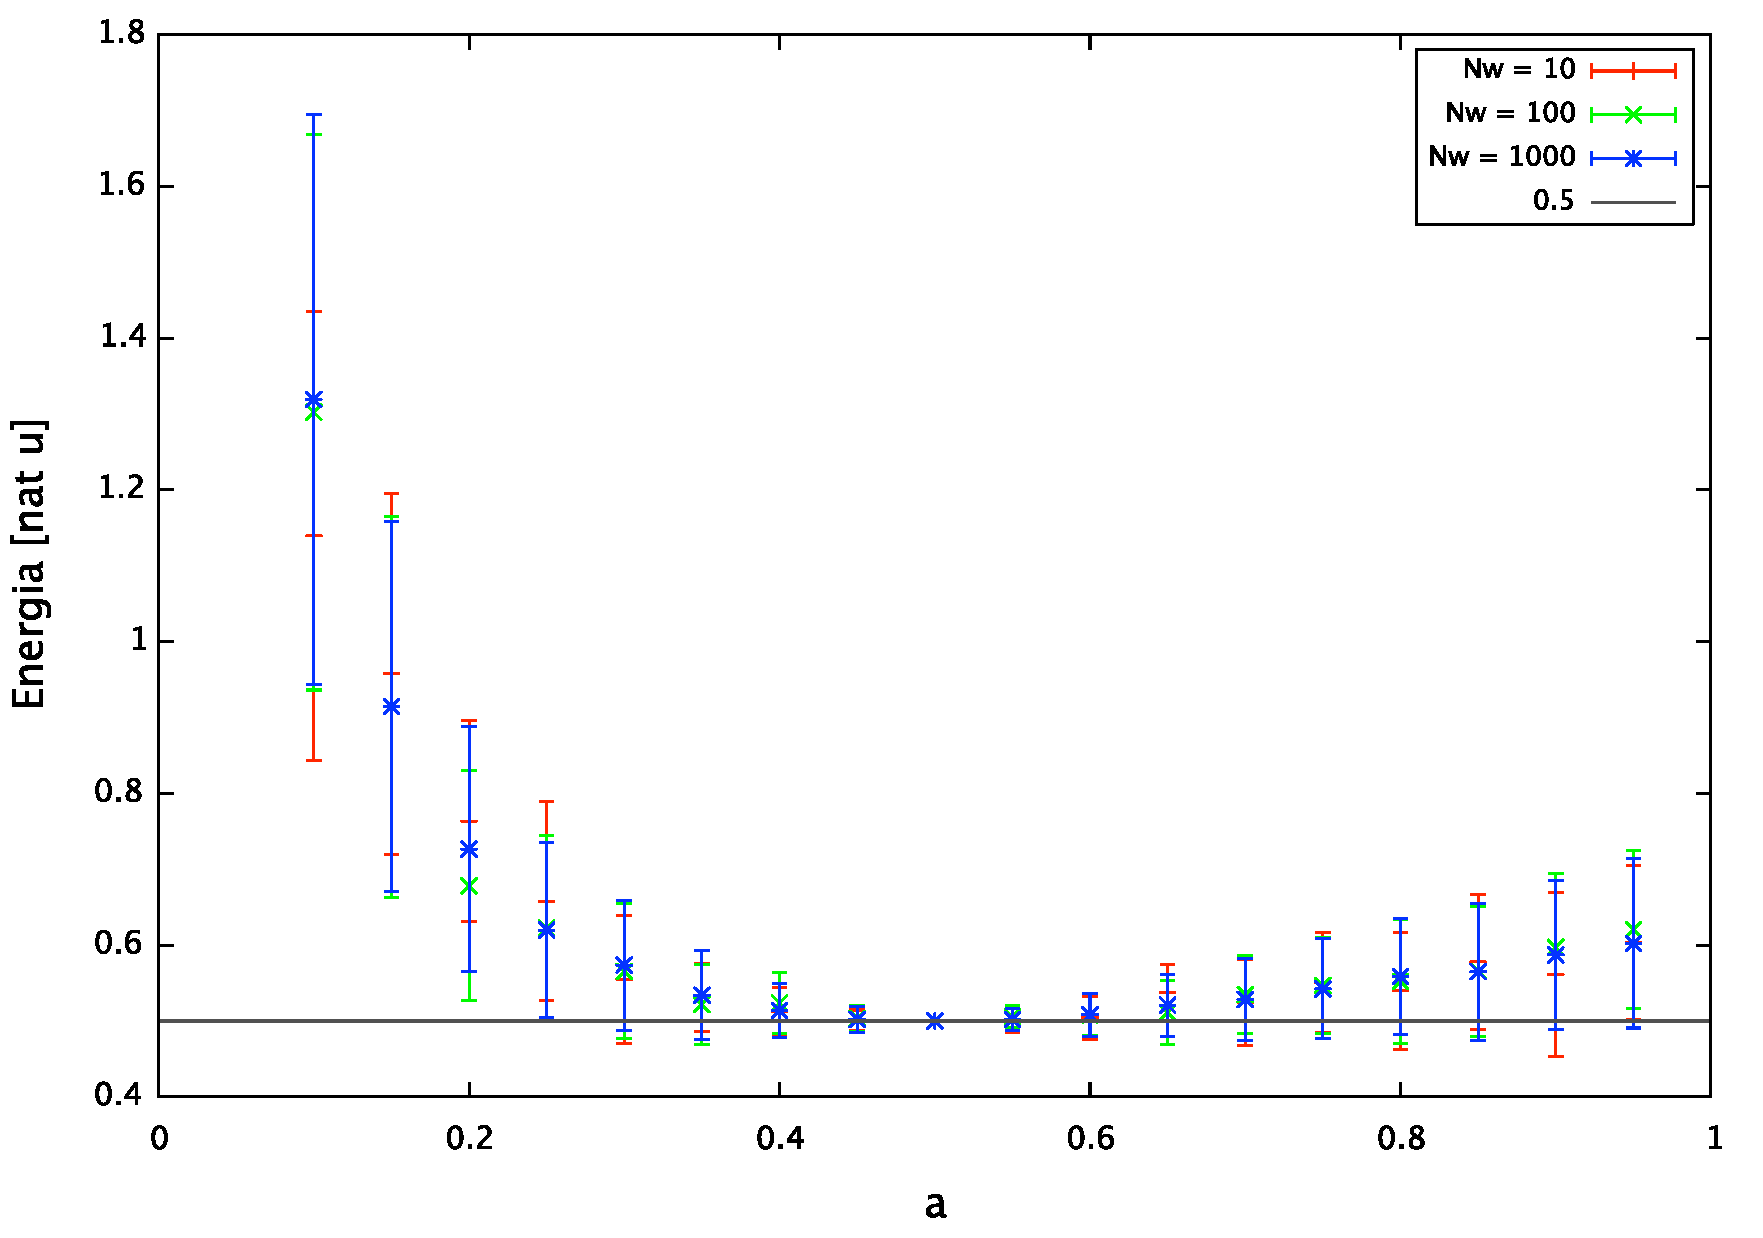
\includegraphics[scale=0.4]{Img/ho_var}
\caption{Andamento di $E_0$ ottenuta tramite VMC al variare di $a$ e di $N_w$}
\end{figure}
Osserviamo che il valore di energia è estremamente impreciso quando il parametro variazionale è molto lontano dal valore corretto, mentre la varianza diminuisce progressivamente avvicinandosi ad $a=1/2$, che ammette varianza nulla. Inoltre, la convergenza al minimo corretto non sembra dipendere dall'energia trial scelta, grazie al meccanismo di aggiornamento di $E_T$ a run-time.\\ L'esistenza del minimo in $a=1/2$ è evidente dall'andamento concavo della funzione $E_0(a)$, anche se esistono, a questo livello di precisione, molti parametri con un'energia compatibile con $E_0^{\text{teorica}}$. E' evidente da Fig. (1) che il problema non è risolto dall'aumento del numero di walkers (che sposta la barra d'errore lasciandone l'ampiezza sostanzialmente invariata), ma piuttosto dall'aumento del tempo di diffusione e dalla diminuzione dello step $\delta \tau$. Con $\delta\tau = 5\times 10^{-5}$, $\tau=50$, $N_w = 20$ e lasciando invariati i restanti parametri si ottengono i risultati in Fig. (2). Alcuni valori significativi di energia corrispondenti alla simulazione mostrata in Fig. (2) sono riportati in Tab. (1). 
\begin{figure}[!h]
\centering
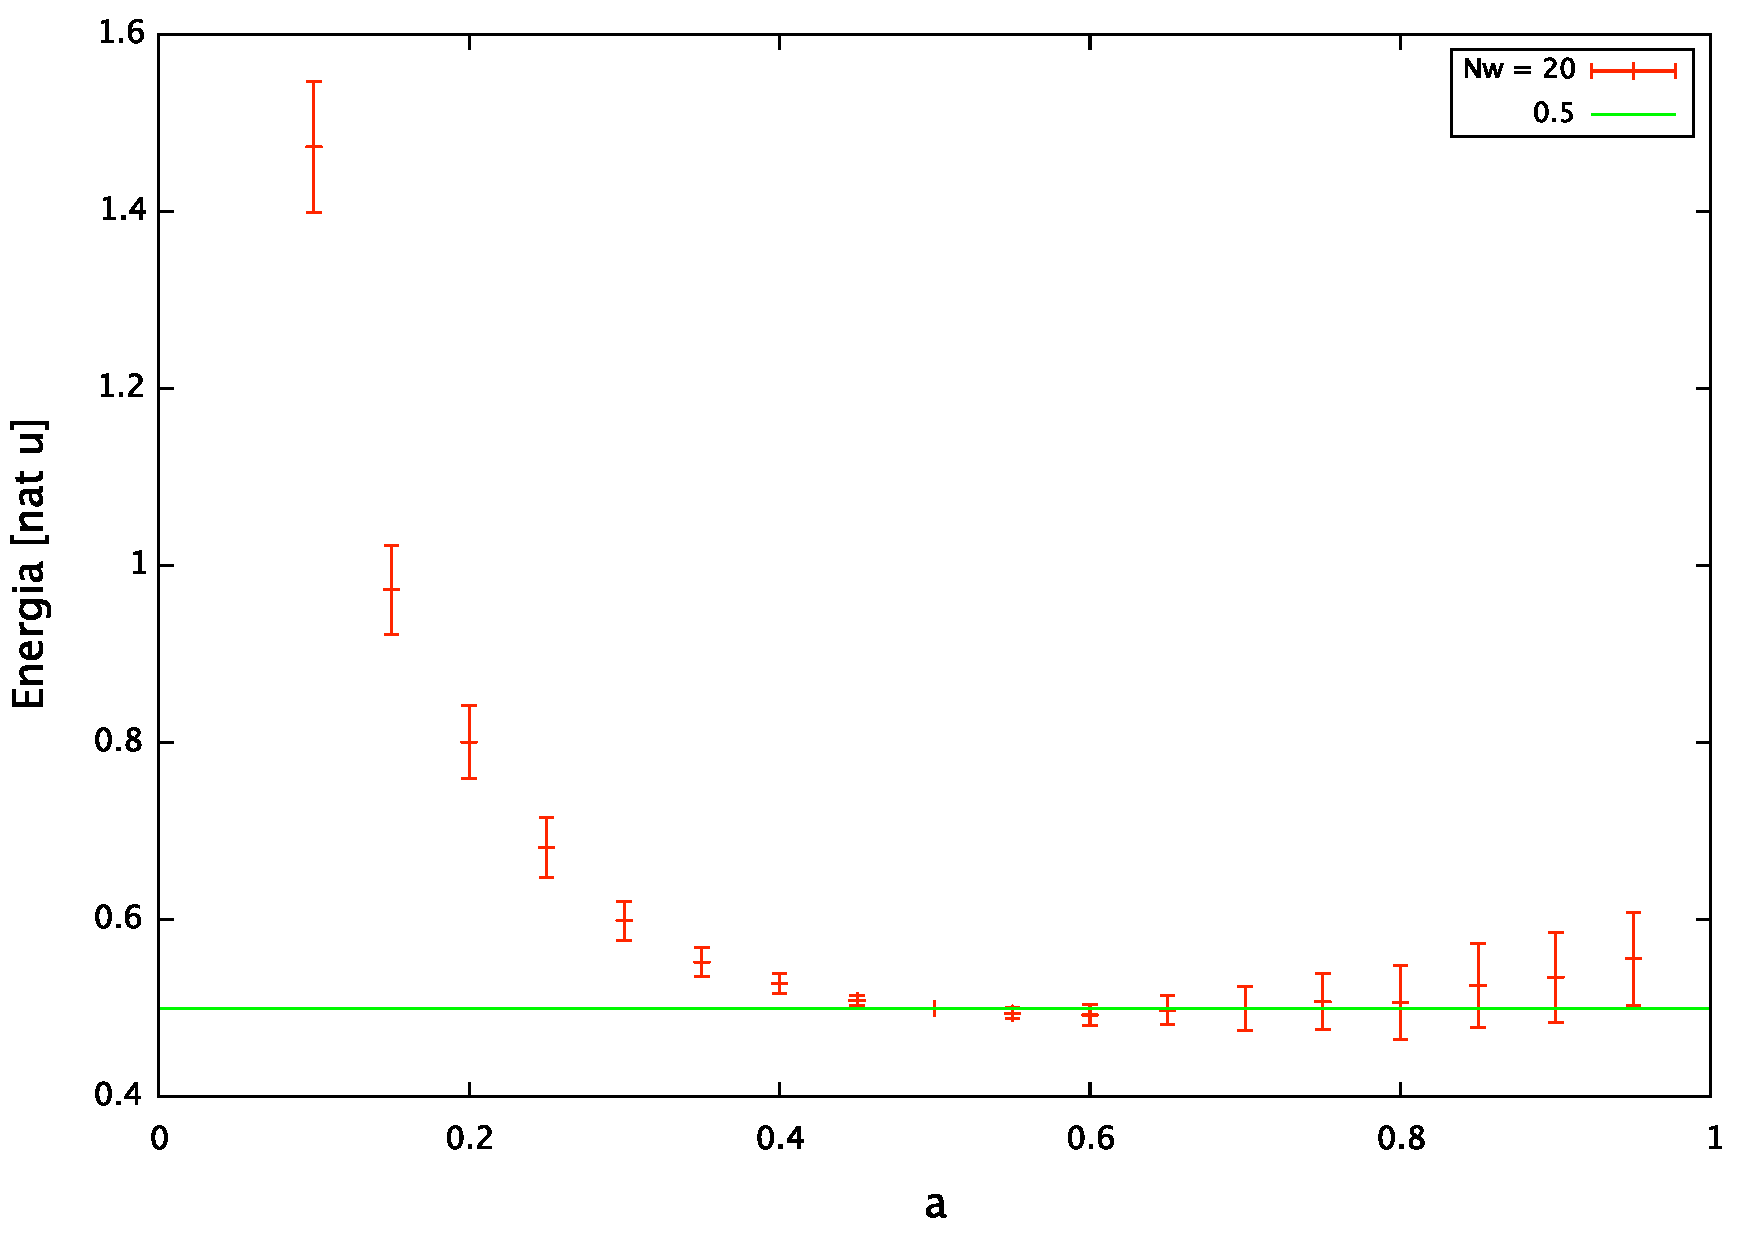
\includegraphics[scale=0.4]{Img/ho_var_good}
\caption{Andamento di $E(a)$ ottenuta tramite VMC con $N_w=20$, $\delta\tau=5\times 10^{-5}$ e $\tau=50$}
\end{figure}
\begin{table}
\centering
\begin{tabular}{|c|c|c|c|c|}
\hline
$a$ & $E_0 \equiv \langle E_{VMC}\rangle$ & $\sigma(E_0)$ & Errore relativo \\ \hline
0.35 & 0.55 & 0.02 & 3.6$\%$ \\ \hline
0.4 & 0.53 & 0.01 & 1.9$\%$\\ \hline
0.45 & 0.509 & 0.006 & 1.2$\%$\\ \hline
0.5 & 0.5000 &	 0 & 0$\%$ \\ \hline
0.55 & 0.495 & 0.006 & 1.2$\%$\\ \hline
0.6 & 0.49 & 0.02 & 4.1$\%$\\ \hline
0.65 & 0.5 	&  0.02 & 4.0$\%$\\ \hline
0.7 &  0.5 &	 0.02 & 4.0$\%$\\ \hline
0.75 & 0.51 &	 0.03 & 5.9$\%$\\ \hline
\end{tabular}
\caption{Valori significativi dell'energia ottenuta tramite VMC per $E_T=1.5$}
\end{table}
E' ragionevole assumere che l'energia minima, ovvero il risultato del calcolo variazionale sia data da
\begin{equation}\label{20}
E_0 = \min_{a}[E(a)+\sigma(E)] - \sigma(E)
\end{equation}
e conseguentemente il risultato del VMC è identico alla previsione teorica per l'energia dell'oscillatore armonico 1D per una particella. \\ \\
Un ulteriore test possibile è quello di utilizzare una funzione d'onda con due parametri ed analizzare l'andamento dell'energia $E(a,b)$ sulla griglia fornita dallo spazio dei parametri considerato. Scegliamo ad esempio
\begin{equation}
\psi_T(x) = e^{-ax^2+bx}
\end{equation}
ed analizziamo lo spazio dei parametri dato da $a\in [0.1,1]$ e $b\in [-0.5,0.5]$. Pseudoforza ed energia locale sono ottenute come
\begin{equation}
\frac{1}{\psi_T(x)} \frac{d\psi_T(x)}{dx} = b-2ax \qquad \frac{1}{\psi_T(x)} \frac{\mathcal{\tilde{H}}\psi_T(x)}{\psi_T(x)} = b^2+4 a^2 x^2-2 a (1+2 b x)
\end{equation}
I risultati ottenuti sono riportati in Fig. (3) e Fig. (4). 
\begin{figure}[!h]
\centering
\subfigure[Proiezione di $E(a,b)$ sugli assi $x-z$]
{\includegraphics[scale=0.25]{Img/Ho_var_3da}}
\hspace{3mm}
\subfigure[Proiezione di $E(a,b)$ sugli assi $y-z$]
{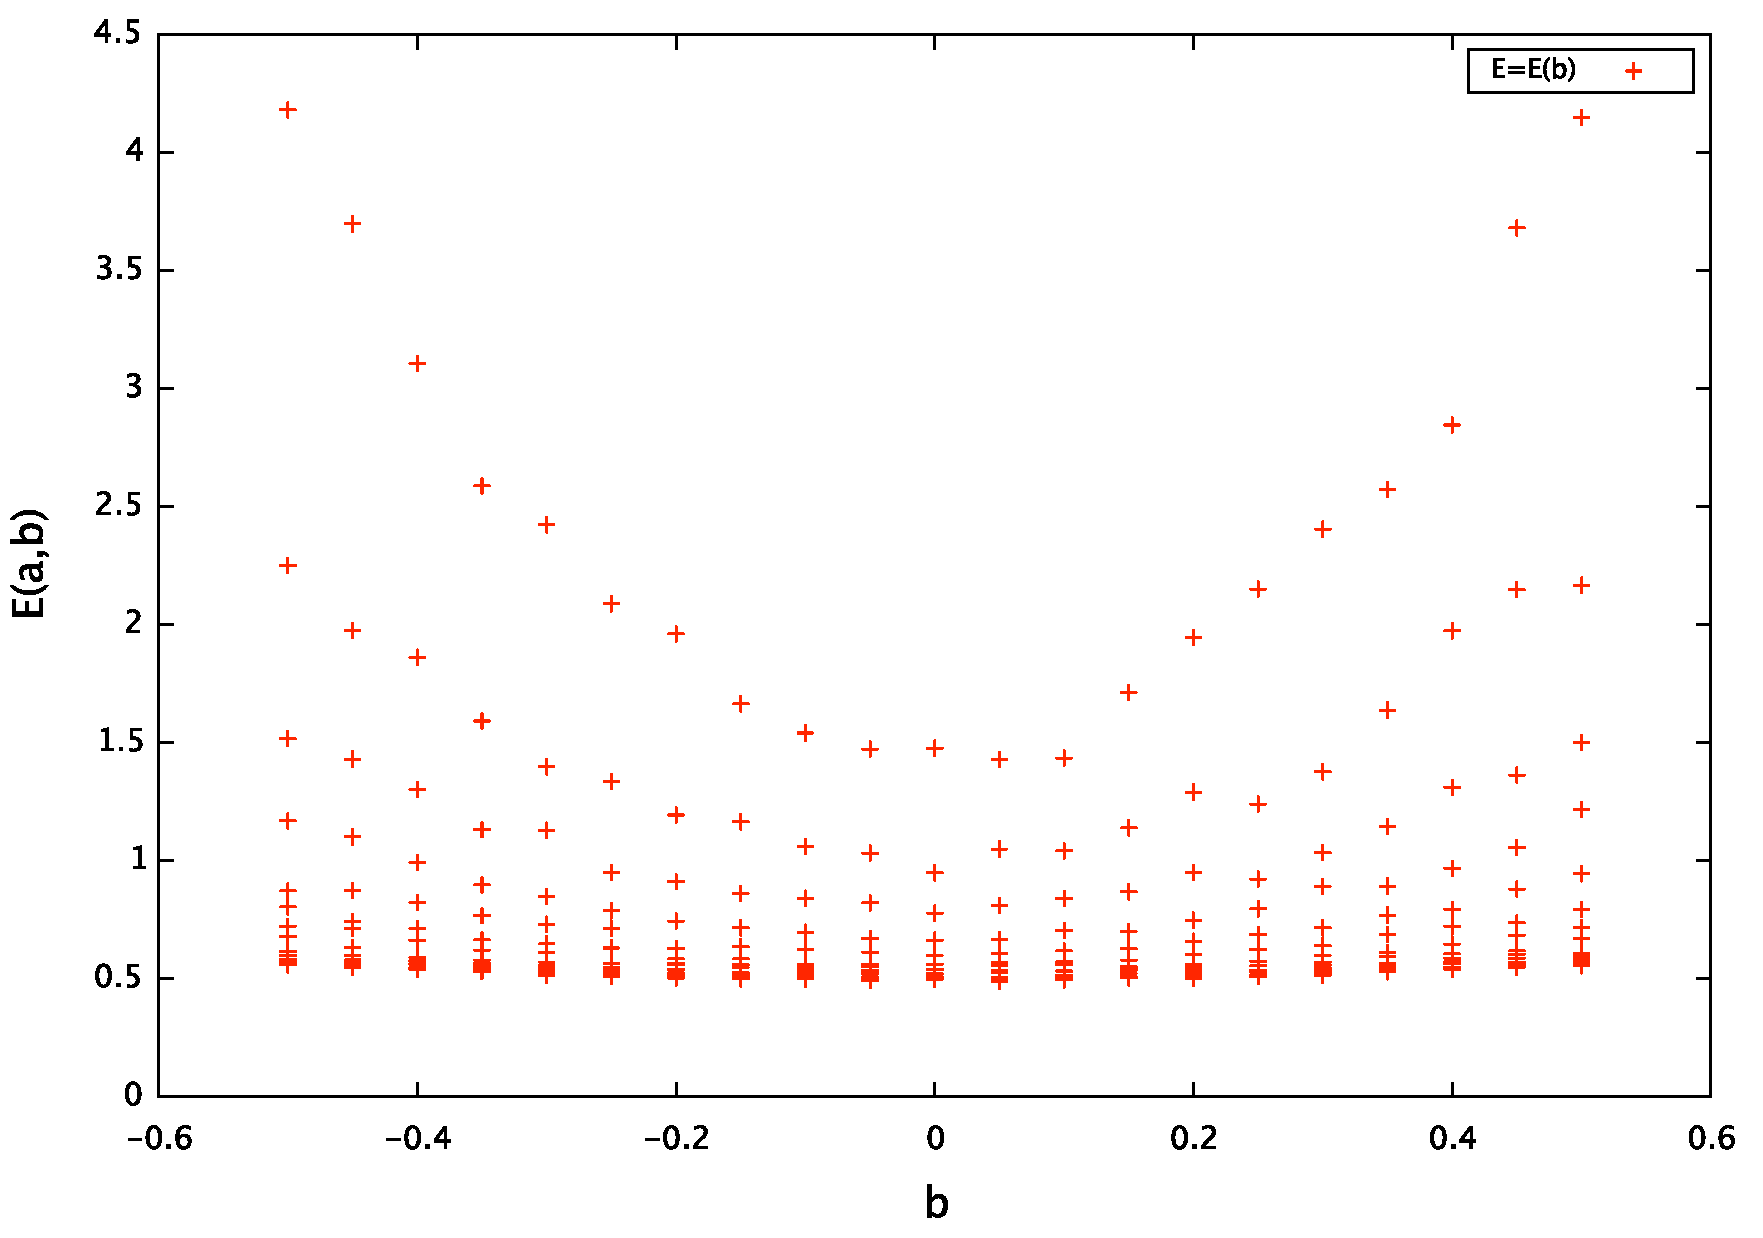
\includegraphics[scale=0.25]{Img/ho_var_3db}}
\caption{Andamento delle proiezioni $E(a,b)$ ottenuta tramite VMC con $N_w=20$, $\delta\tau=5\times 10^{-5}$ e $\tau=50$}
\end{figure}
\begin{figure}[!h]
\centering
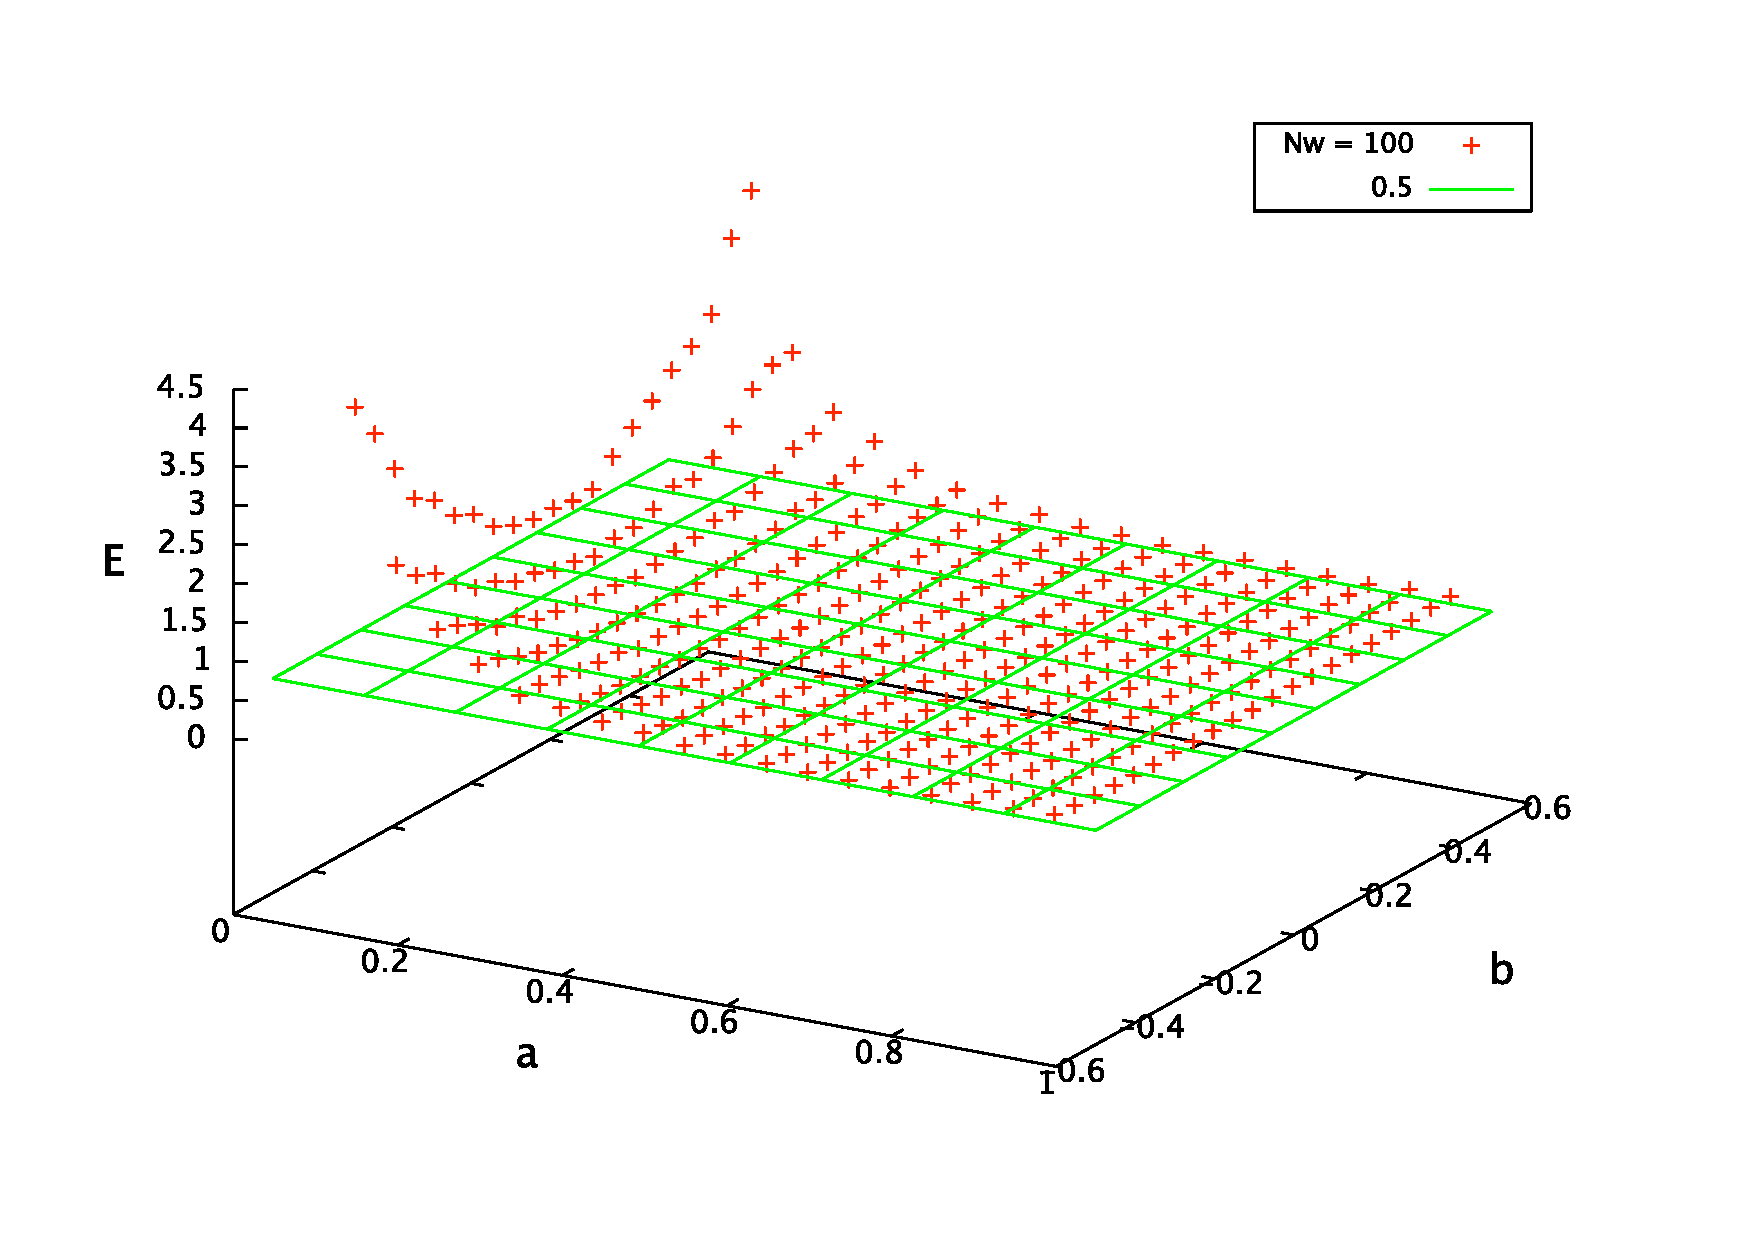
\includegraphics[scale=0.35]{Img/ho_var_3d}
\caption{Andamento di $E(a)$ ottenuta tramite VMC con $N_w=20$, $\delta\tau=5\times 10^{-5}$ e $\tau=50$}
\end{figure}
Alcuni valori significativi di energia corrispondenti alla simulazione mostrata in Fig. (3) - Fig. (4) sono riportati in Tab. (2).  
\begin{table}
\centering
\begin{tabular}{|c|c|c|c|c|c|}
\hline
$a$ & $b$ &$E_0 \equiv \langle E_{VMC}\rangle$ & $\sigma(E_0)$ & Errore relativo \\ \hline
0.5 &	 -0.2& 	 0.520 &	 0.006 & 1.2$\%$ \\ \hline
0.5  & -0.15 	& 0.512 &	 0.005 & 1.0$\%$ \\ \hline
0.5 	& -0.1 	 &0.507 	& 0.003 & 0.6$\%$ \\ \hline
0.5 	& -0.05 &	 0.501 &	 0.001 & 0.2$\%$ \\ \hline
0.5 	& 0 & 	 0.5000 	& 0 & 0$\%$ \\ \hline
0.5 	& 0.05 & 	 0.501 &	 0.001 & 0.2$\%$ \\ \hline
0.5 	& 0.1 	& 0.505 	& 0.003& 0.6$\%$ \\ \hline
0.5 	& 0.15 	& 0.511 &	 0.005 & 1.0$\%$ \\ \hline
0.5 	& 0.2 	& 0.522 	& 0.006 & 1.2$\%$ \\ \hline
\end{tabular}
\caption{Valori significativi dell'energia ottenuta tramite VMC per $E_T=1.5$}
\end{table}
Utilizzando nuovamente il criterio stabilito in \eqref{20} possiamo dedurre che i parametri variazionali ottimali sono dati da $a=0.5$ e $b=0$, da cui deriva un'energia $E_0^{calc}=0.5$ identica all'aspettativa teorica. \\ \\
Una volta verificata la bontà dei risultati del VMC possiamo passare a discutere quelli del DMC. Il DMC è di per sè un metodo robusto, che riesce a convergere a valori molto ragionevoli di energia anche quando il risultato variazionale di partenza non è di particolare qualità. Questo si può vedere chiaramente dal grafico in Fig. (5), dove sono stati utilizzati $\delta\tau = 5\times 10^{-5}$, $\tau_{\text{VMC}}=25$, $\tau_{\text{DMC}}=50$, $N_w = 100$ e $E_T=1.5$. Fig. (6) e Fig. (7) mostrano invece l'andamento del numero di walkers e dell'energia in funzione dei cicli DMC svolti (l'incertezza sull'energia non viene mostrata per ragioni di chiarezza del grafico), utilizzando gli stessi parametri precedentemente descritti. I valori della popolazione di walkers vengono raccolti ogni 200 cicli, mentre quelli di energia ogni 1000 cicli. Osserviamo che la popolazione di walkers rimane ragionevolmente costante lungo la diffusione, come previsto attraverso l'inserimento dei pesi statistici riscalati, mentre l'energia fluttua sensibilmente circa per i primi 400.000 cicli, stabilizzandosi dopo e convergendo all'energia attesa. La fluttuazione dell'energia è ovviamente una caratteristica attesa, data la natura statistica dell'algoritmo. 
\begin{figure}[!h]
\centering
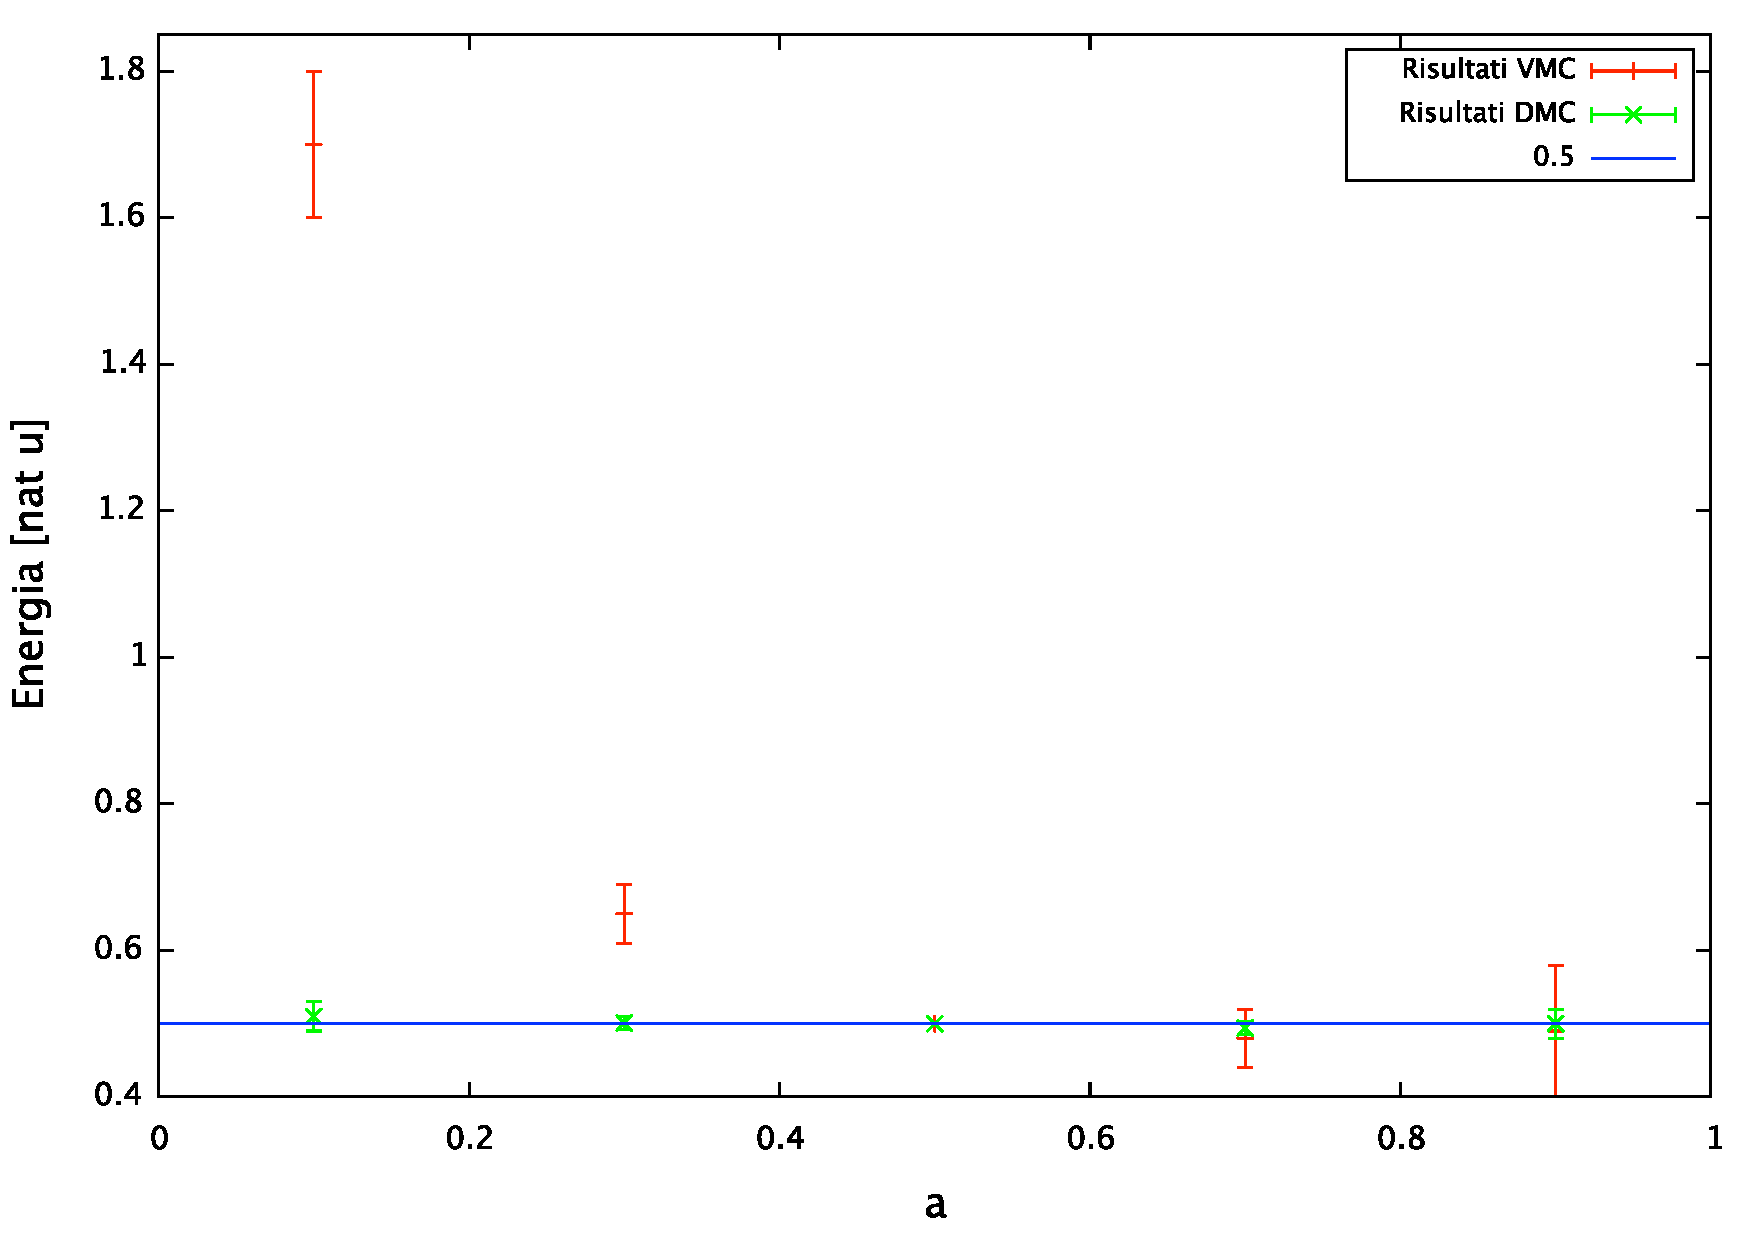
\includegraphics[scale=0.4]{Img/dmc_var}
\caption{Confronto tra i risultati del VMC e del DMC al variare di $a$}
\end{figure}
\begin{figure}[!h]
\centering
\subfigure[$a=0.1$ ed $E_T = 1.7$]
{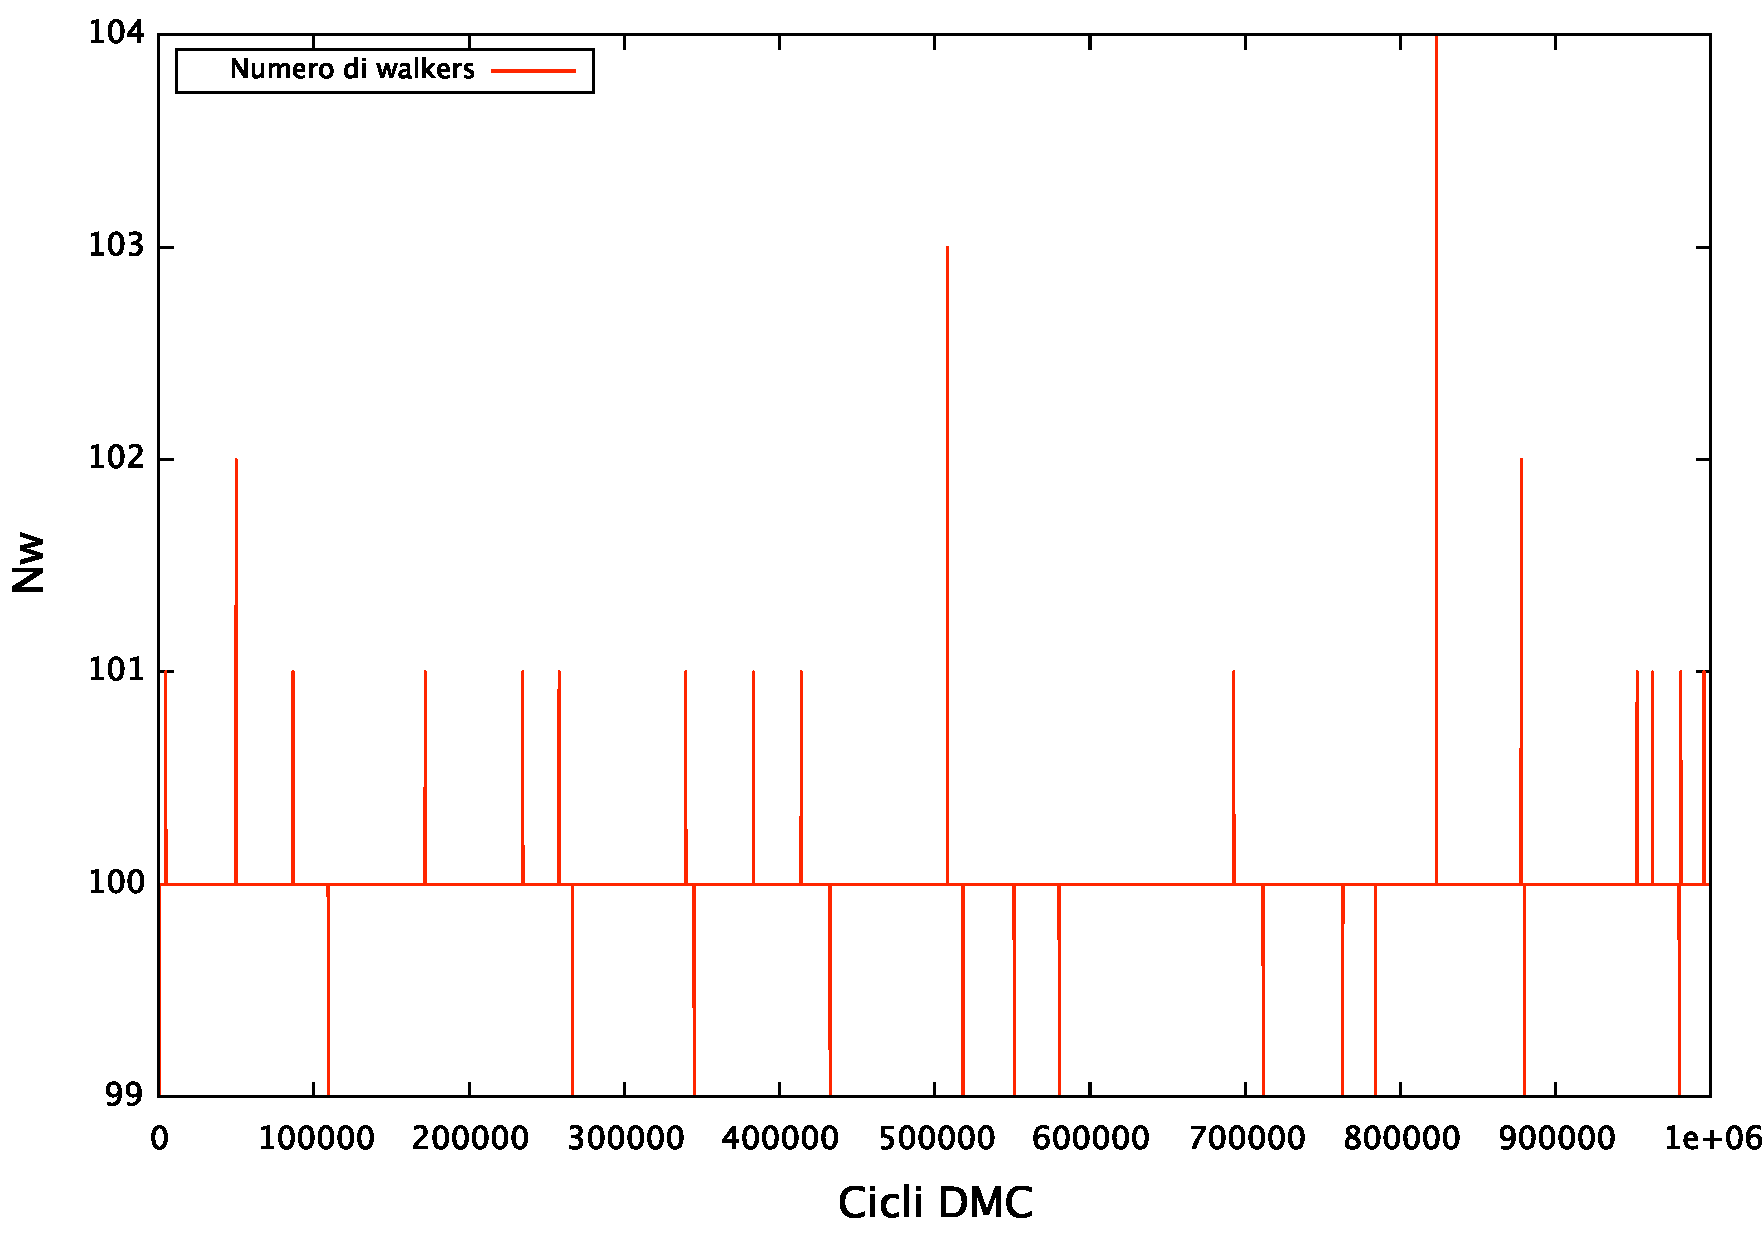
\includegraphics[scale=0.25]{Img/nw_01}}
\hspace{3mm}
\subfigure[$a=0.3$ ed $E_T=0.65$]
{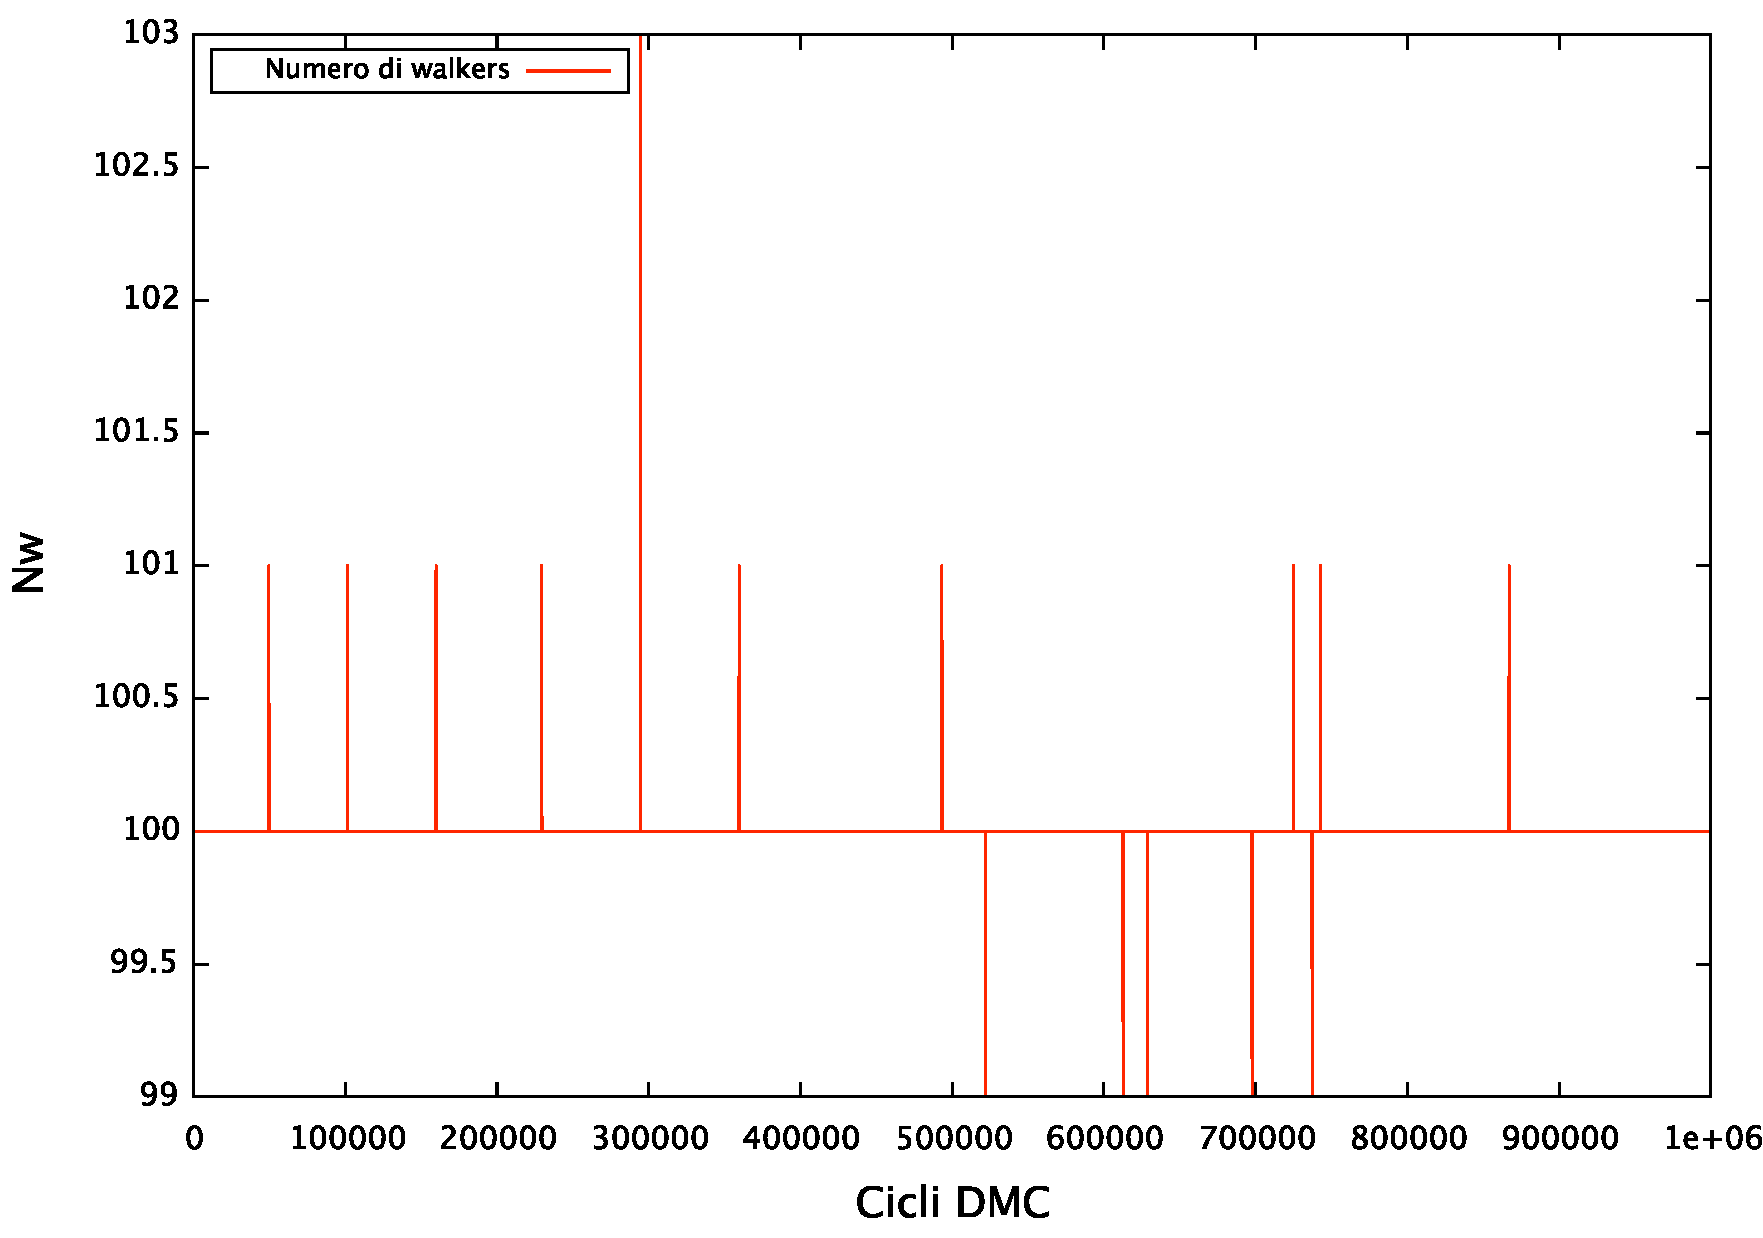
\includegraphics[scale=0.25]{Img/nw_03}}
\hspace{3mm}
\subfigure[$a=0.5$ ed $E_T=0.5$]
{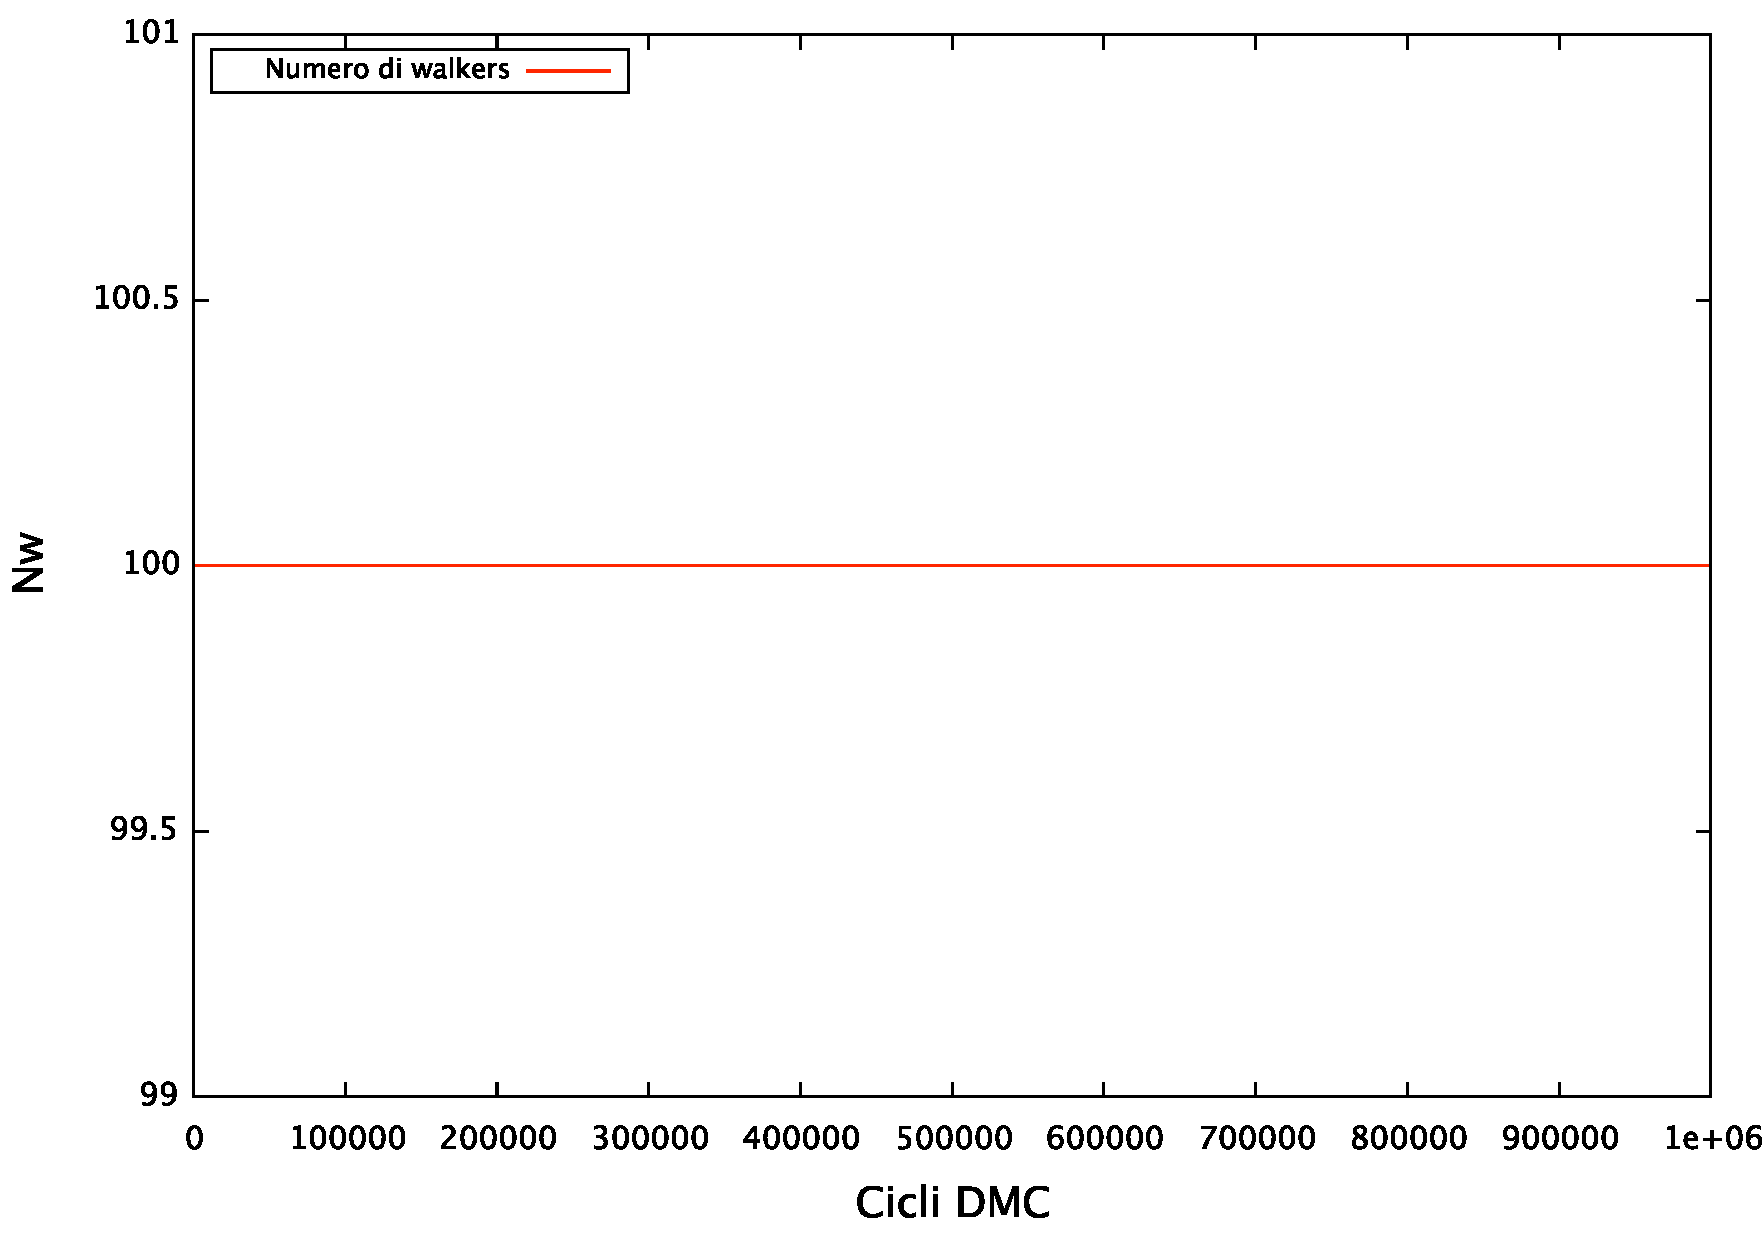
\includegraphics[scale=0.25]{Img/nw_05}}
\hspace{3mm}
\subfigure[$a=0.7$ ed $E_T=0.48$]
{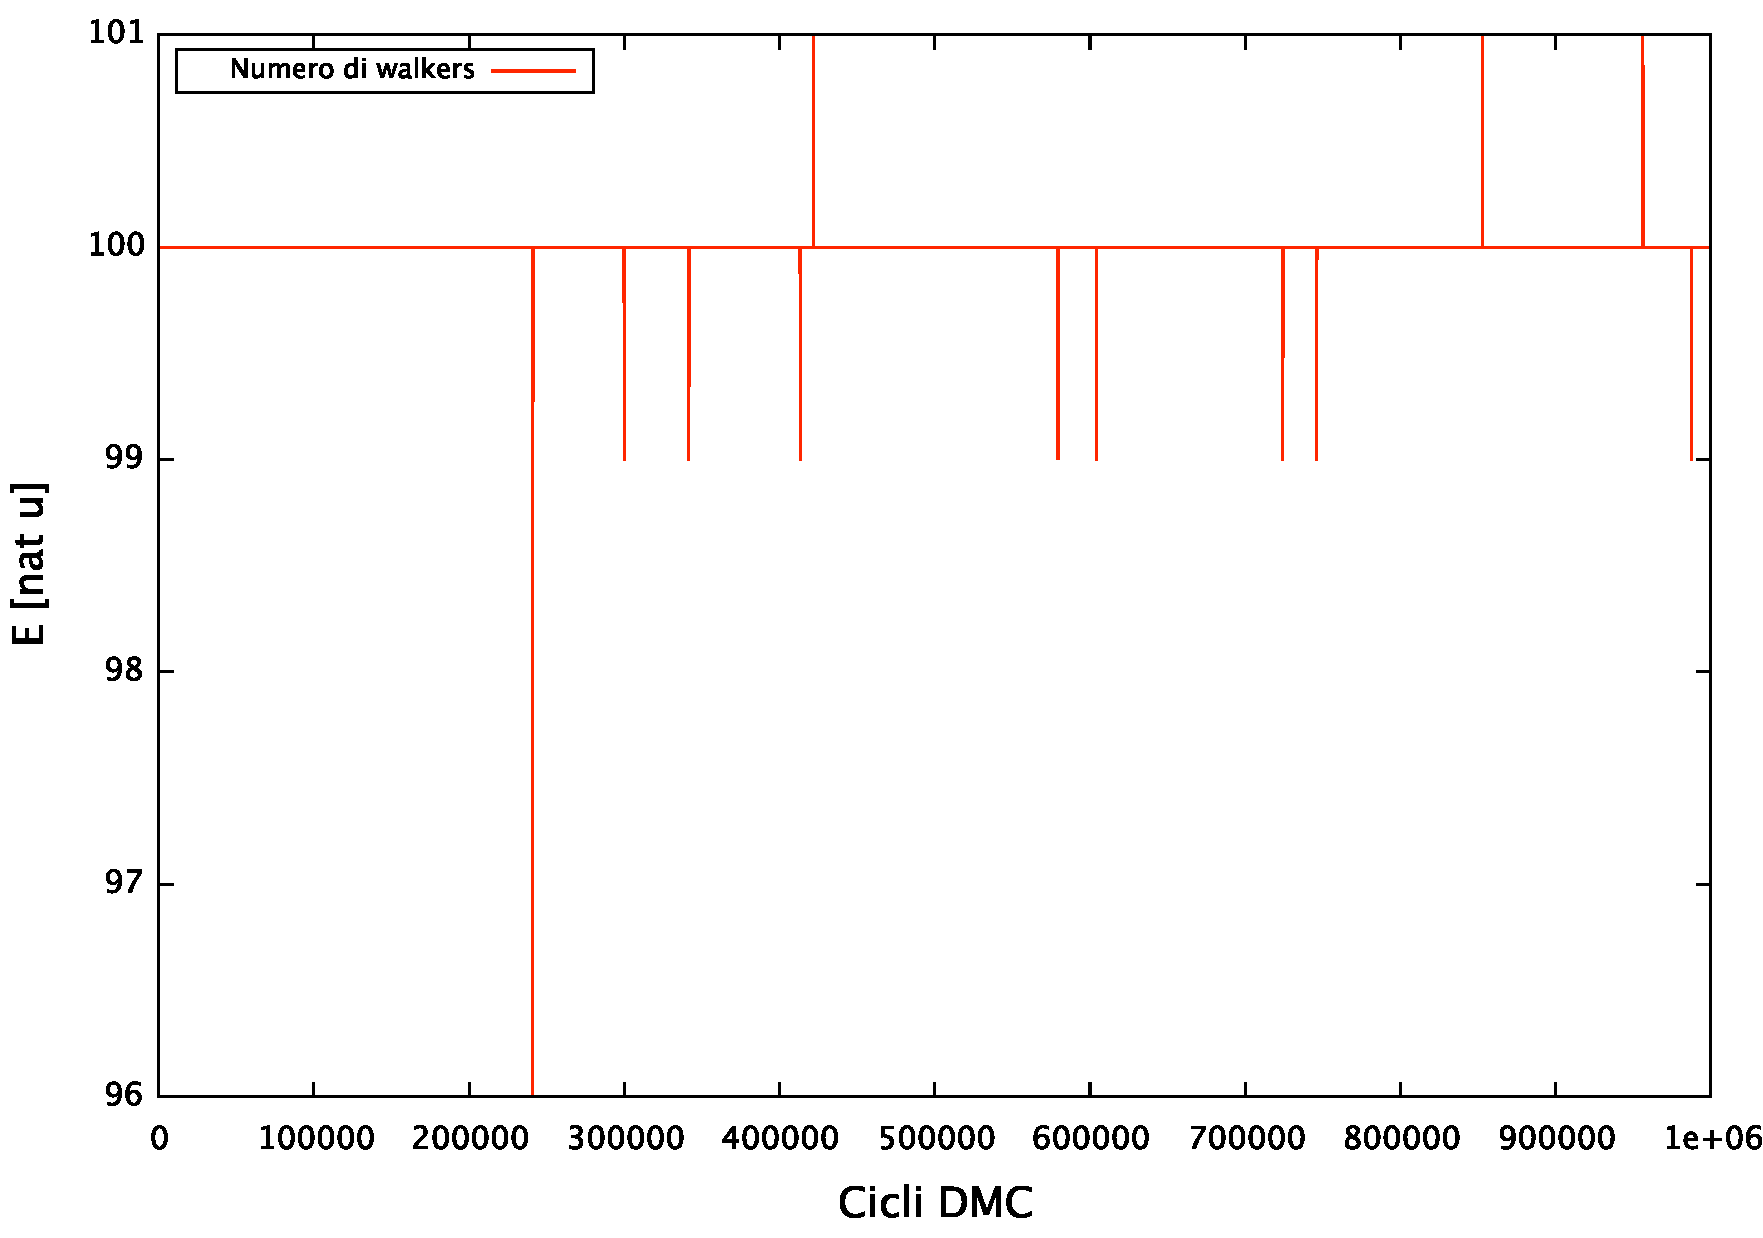
\includegraphics[scale=0.25]{Img/nw_07}}
\caption{Andamento del numero di walkers per la diffusione con diversi $a$ ed $E_T=\langle E_{VMC}\rangle$}
\end{figure}
\begin{figure}[!h]
\centering
\subfigure[$a=0.1$ ed $E_T = 1.7$]
{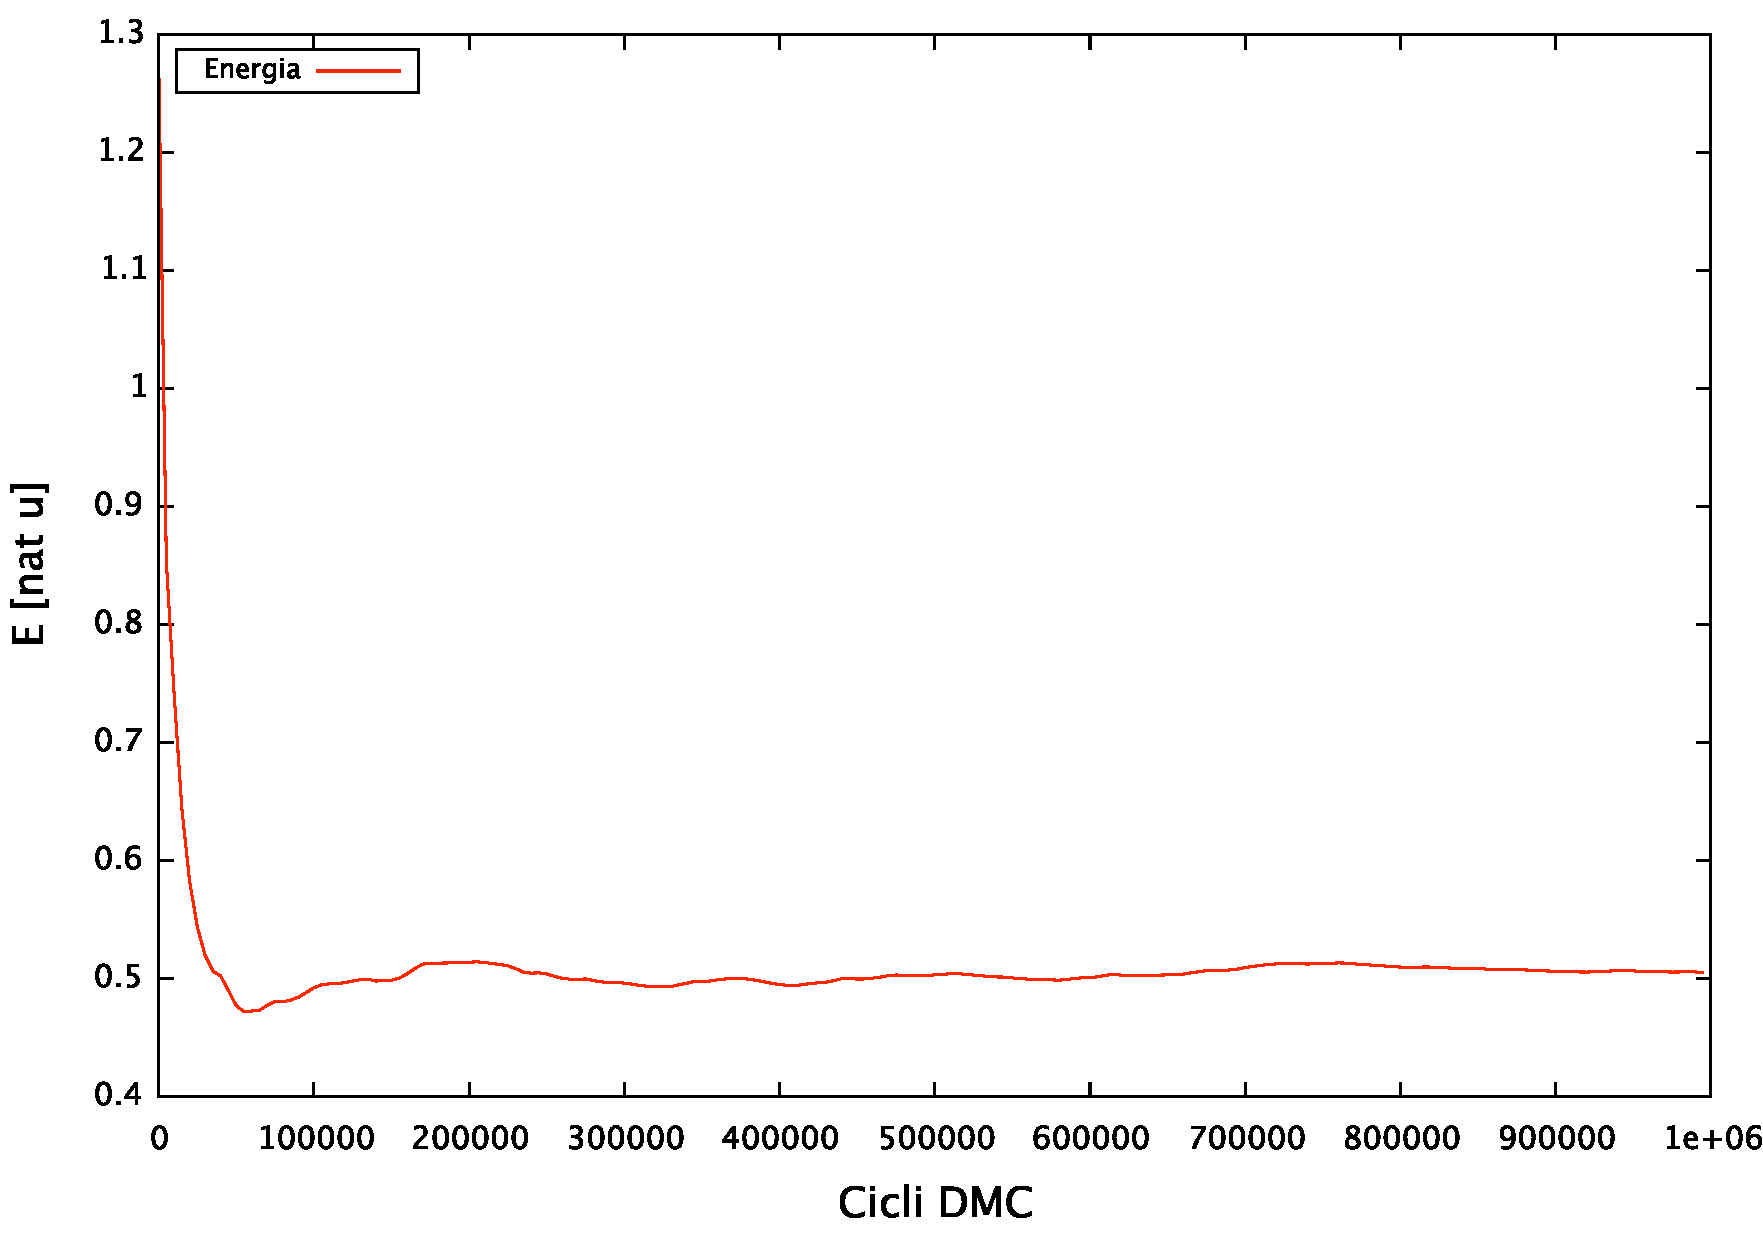
\includegraphics[scale=0.25]{Img/e_01}}
\hspace{3mm}
\subfigure[$a=0.3$ ed $E_T=0.65$]
{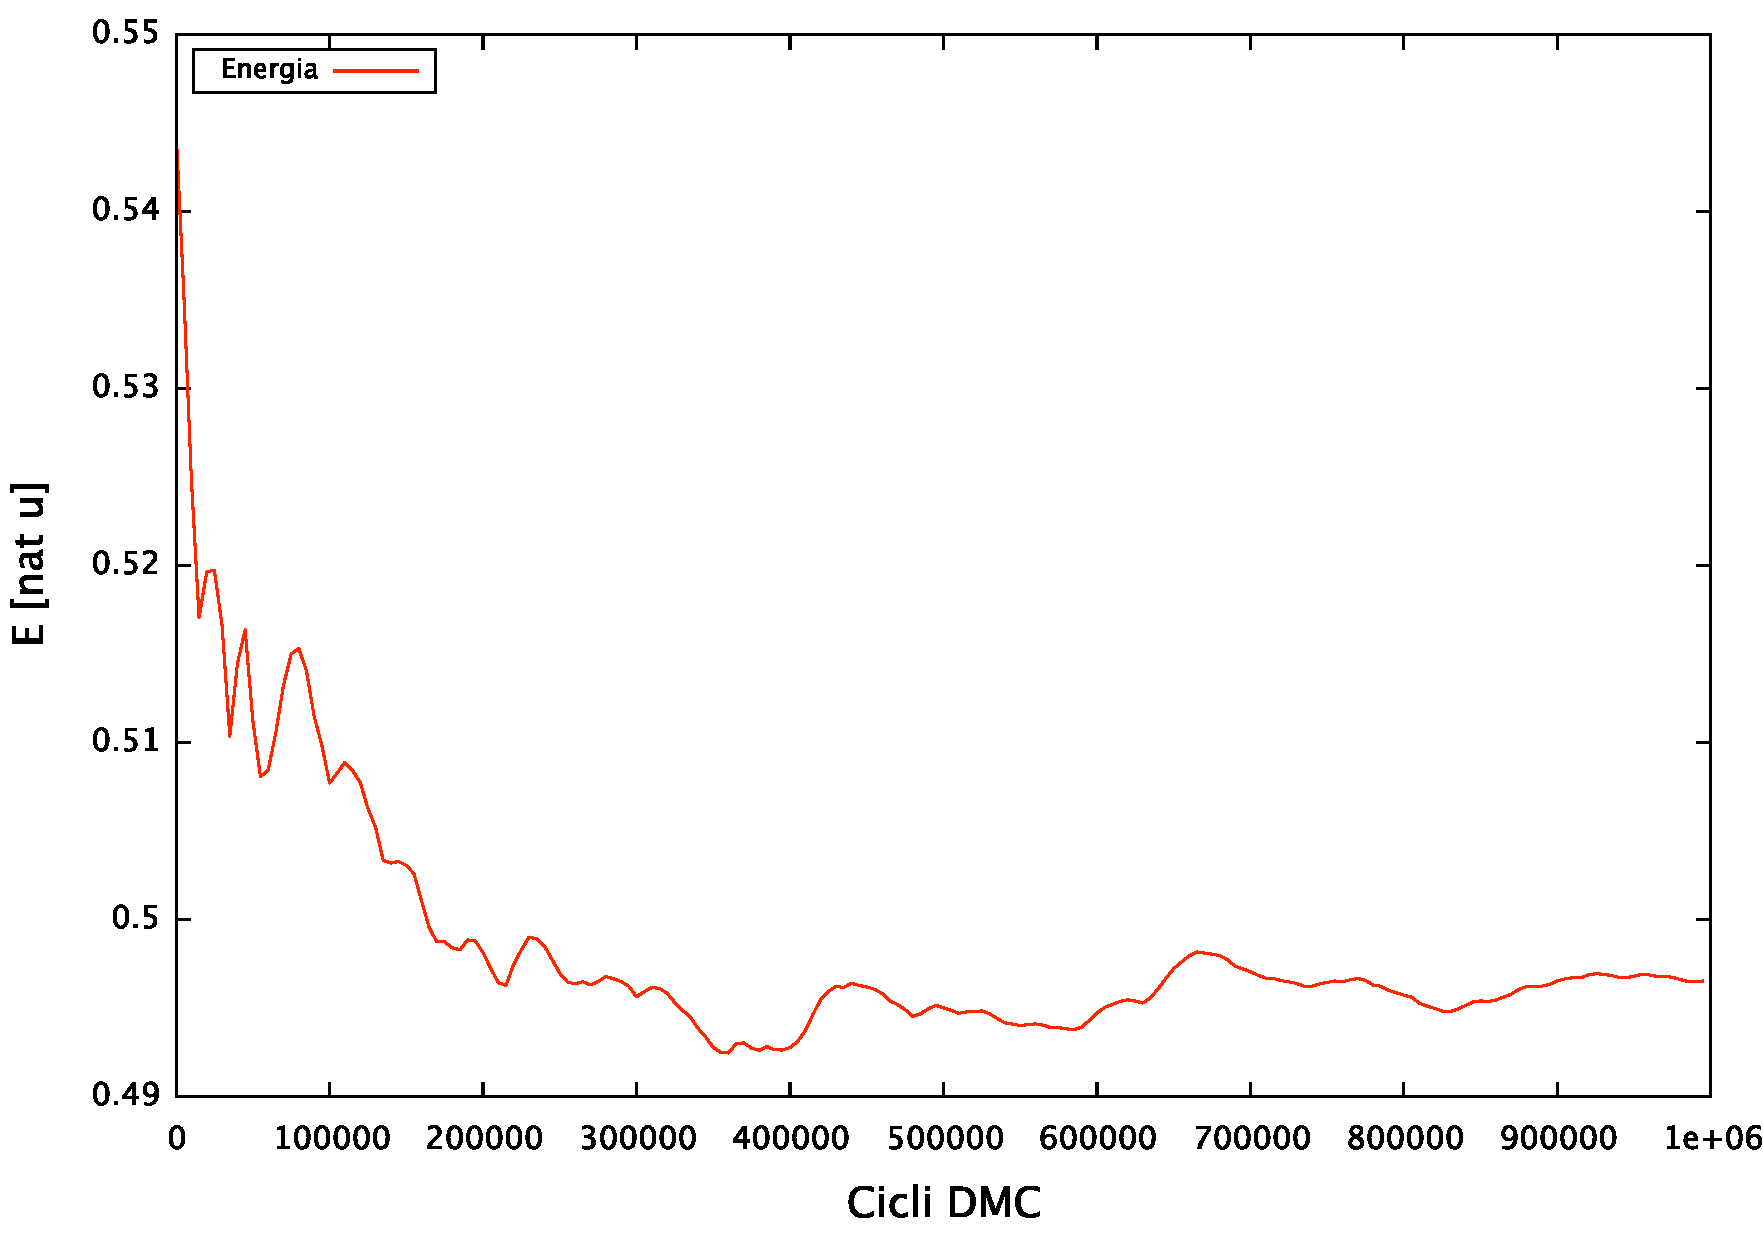
\includegraphics[scale=0.25]{Img/e_03}}
\hspace{3mm}
\subfigure[$a=0.5$ ed $E_T=0.5$]
{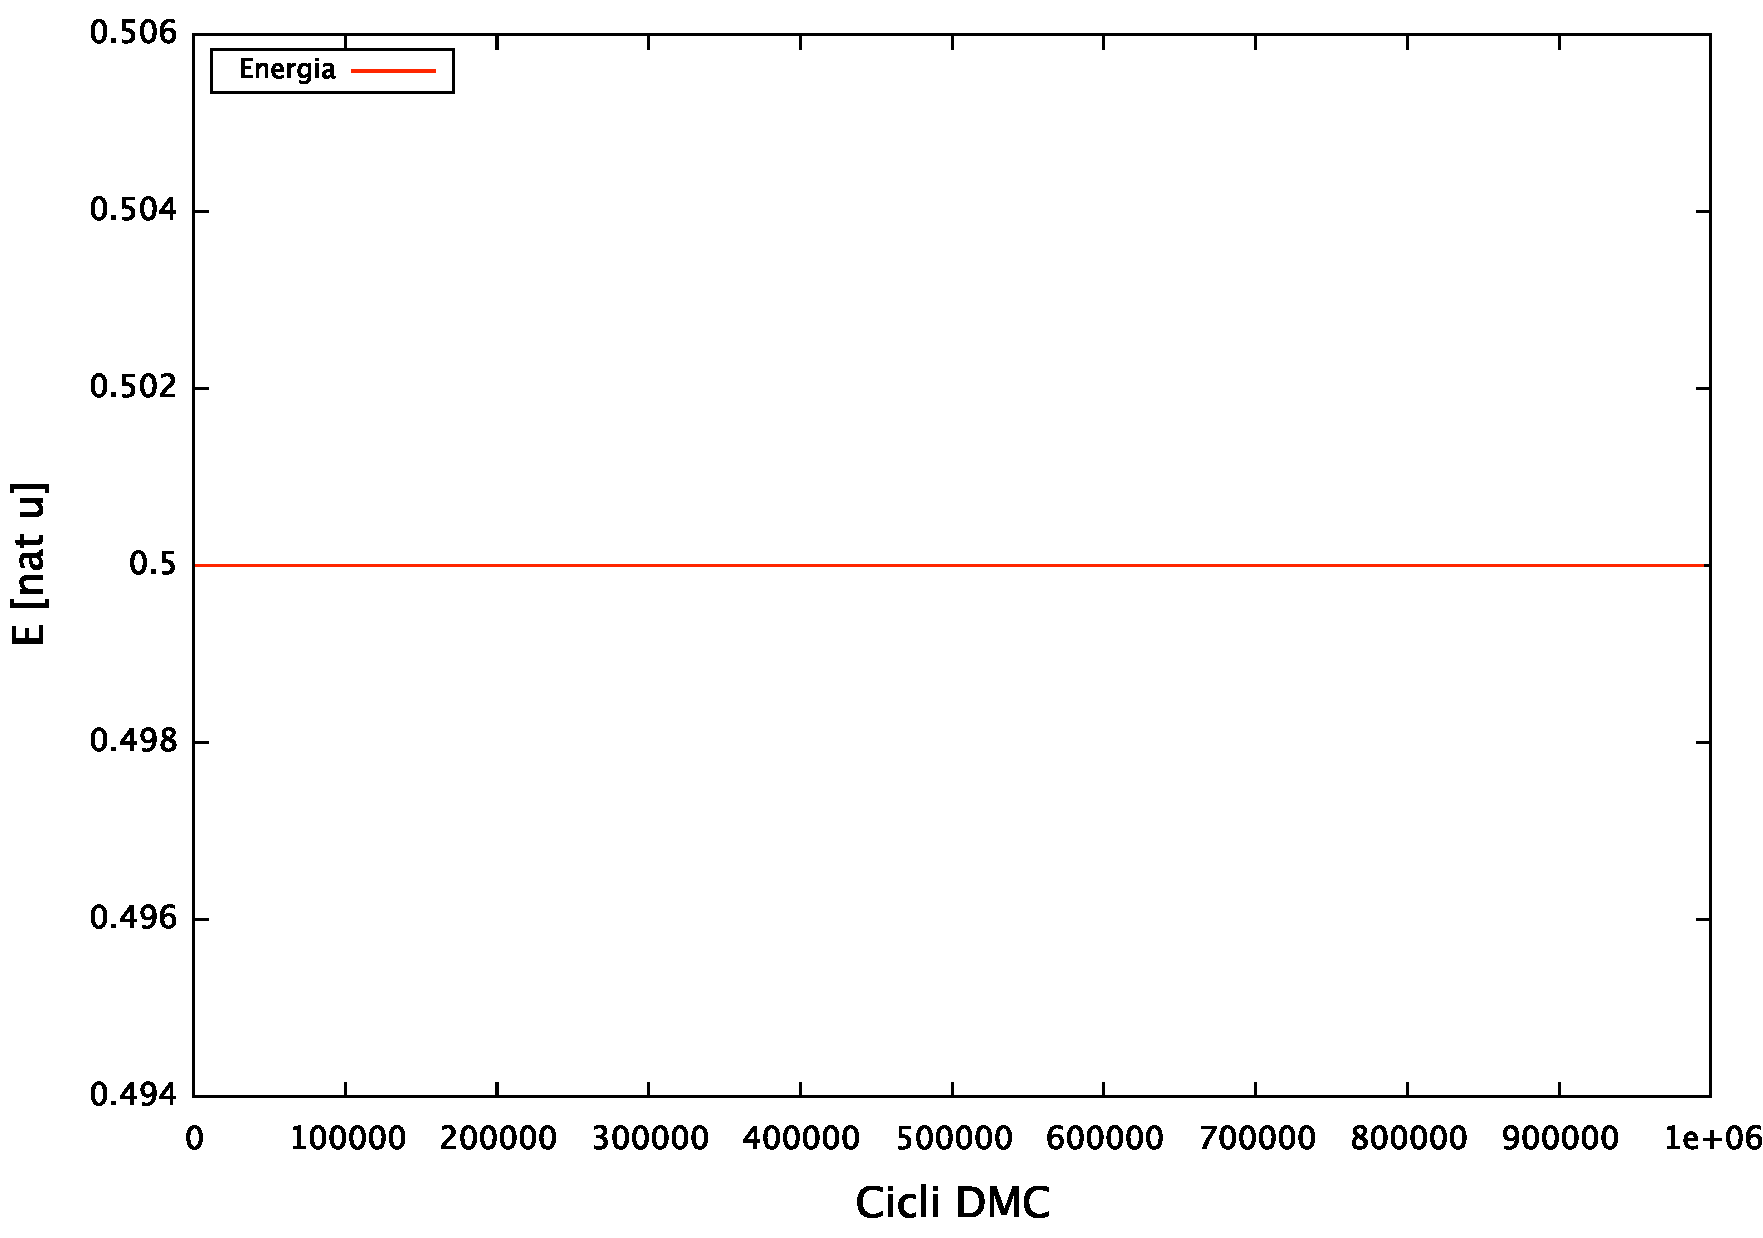
\includegraphics[scale=0.25]{Img/e_05}}
\hspace{3mm}
\subfigure[$a=0.7$ ed $E_T=0.48$]
{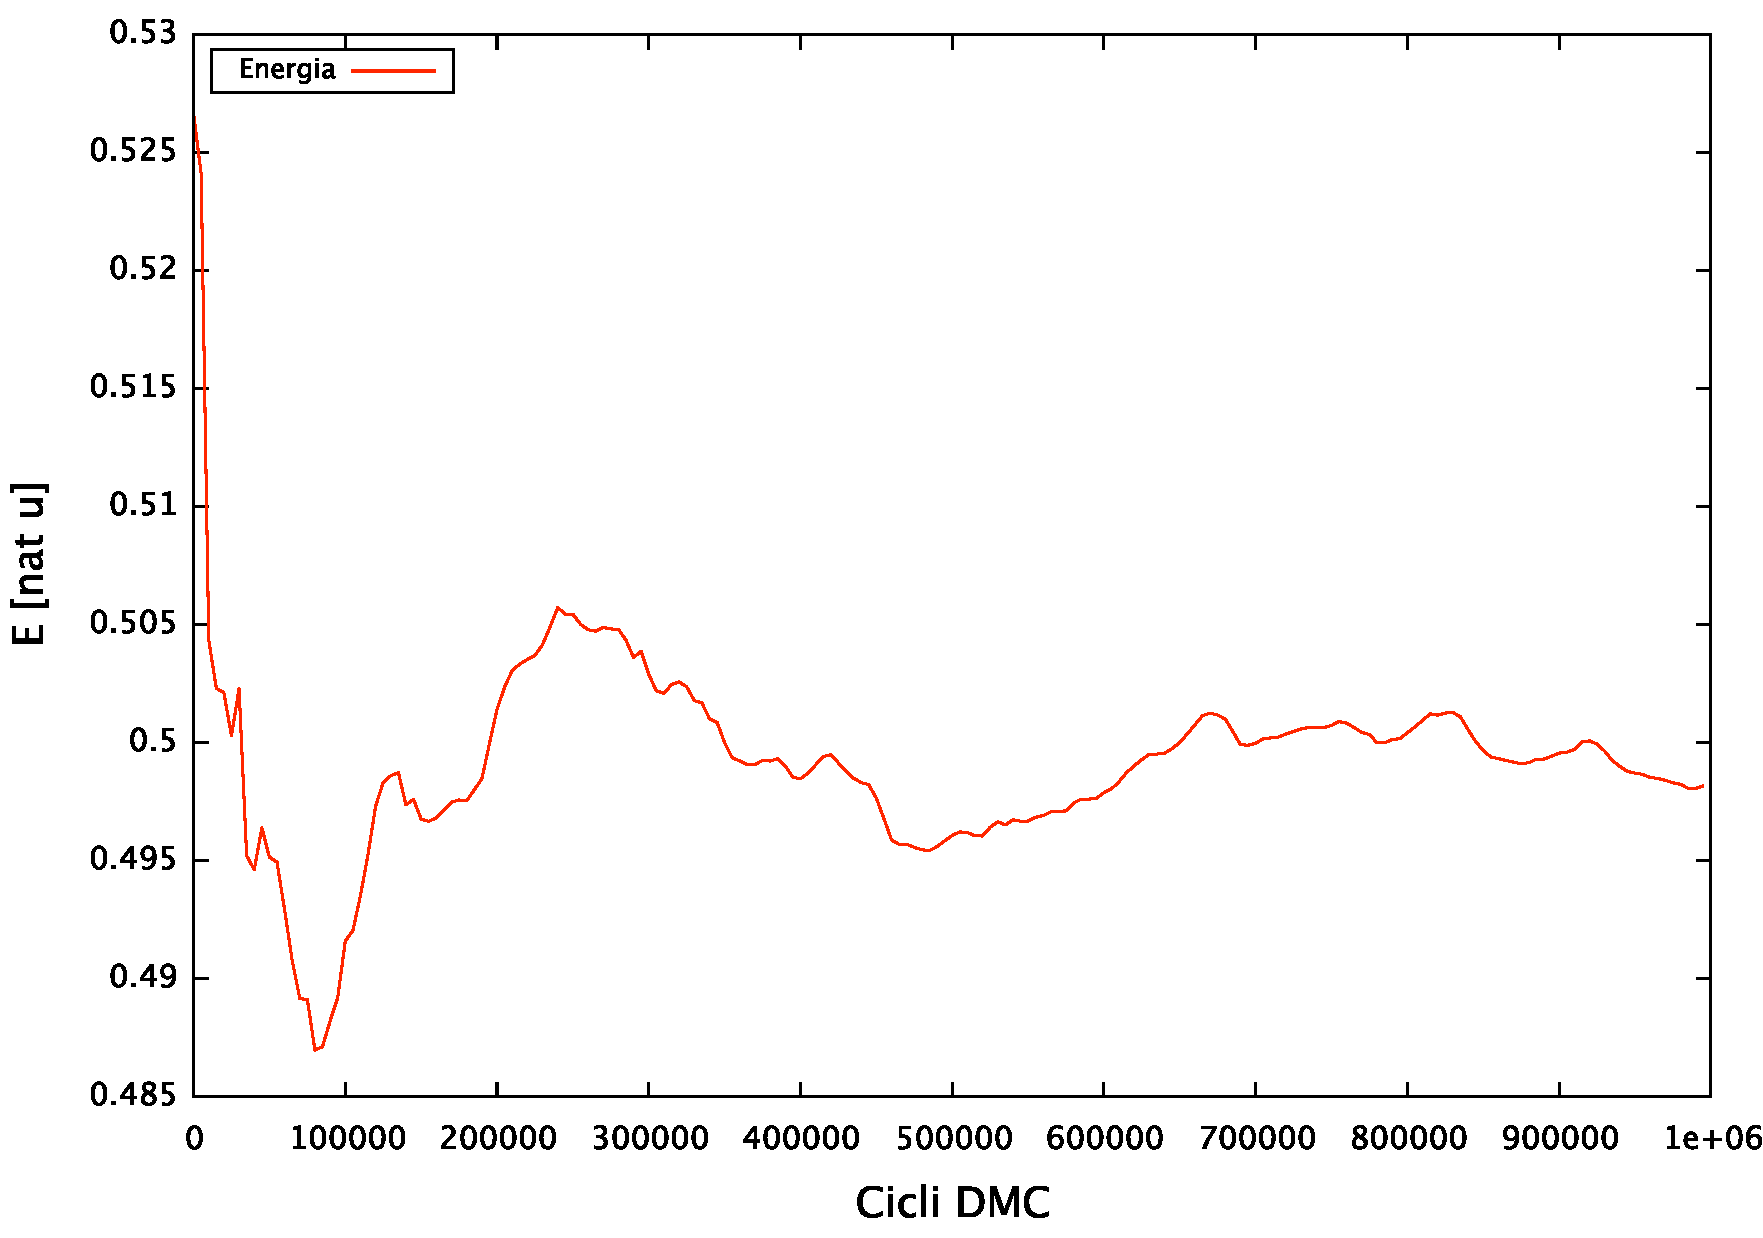
\includegraphics[scale=0.25]{Img/e_07}}
\caption{Andamento dell'energia con diversi $a$ ed $E_T=\langle E_{VMC}\rangle$}
\end{figure}\
\newpage
Un utile check di consistenza dell'algoritmo DMC è mostrato in Fig. (6)-c e Fig. (7)-c, dove come input iniziale per il Diffusion Monte Carlo vengono inseriti l'energia trial ed il parametro varizionale esatti. In questo caso, come atteso, il numero di walkers non cambia mai ed anche l'energia rimane costante al valore iniziale, confermando le nostre aspettative. 

\subsection{N particelle in 3 dimensioni}
Nel caso più generale delle N particelle in 3 dimensioni abbiamo che l'Hamiltoniana ridotta è data da
\begin{equation}
\mathcal{\tilde{H}} = -\frac{1}{2}\sum_{i=1}^N \nabla^2_i + \frac{1}{2}\sum_{i=1}^N\textbf{r}_i^2
\end{equation}
Sulla falsa riga della trattazione semplificata, una buona funzione d'onda guess è data da
\begin{equation}
\psi_T(\textbf{r}_1, \ldots, \textbf{r}_N) = e^{-a\sum_{i=1}^N \textbf{r}_i^2}
\end{equation}
Energia locale e pseudoforza si ottengono derivando termine a termine la funzione d'onda
\begin{equation}
\frac{\boldsymbol{\nabla}_i\psi_T(R)}{\psi_T(R)} = -2a\textbf{r}_i \qquad \frac{\mathcal{\tilde{H}}\psi_T(R)}{\psi_T(R)} = \sum_{i=1}^N (3a - 2\textbf{r}_i^2a^2 + \frac{1}{2}\textbf{r}_i^2)
\end{equation}
Nelle precedenti simulazioni abbiamo ignorato il fatto che alcuni valori di energia scendono, in assoluto, sotto il valore di energia del ground state, ma rimangono compatibili con il valore teorico entro l'incertezza. Questo è dovuto al fatto che nei primissimi cicli di VMC l'energia cala bruscamente dal valore trial ad un valore simile a quello corretto e oscilla notevolmente, fino poi a stabilizzarsi. Una pratica diffusa (anche quando si utilizza l'algoritmo di Metropolis, ad esempio) è quella di cominciare a sommare i contributi all'energia dopo una certa soglia di stabilizzazione. Nel problema 3D è stato dunque implementato questo approccio, \emph{termalizzando} il sistema per $\tau_{\text{term}} = 10$ e diffondendo poi fino a $\tau=40$. In Fig. (8) vengono mostrati i risultati rispettivamente per 1, 2, 5 e 10 oscillatori armonici 3D disaccoppiati, dove sono stati utilizzati i seguenti parametri: $\delta \tau = 5\times 10^{-5}$, $N_w=50$, $E_T = 3.0$. 
 \begin{figure}[!h]
\centering
\subfigure[$N=1$]
{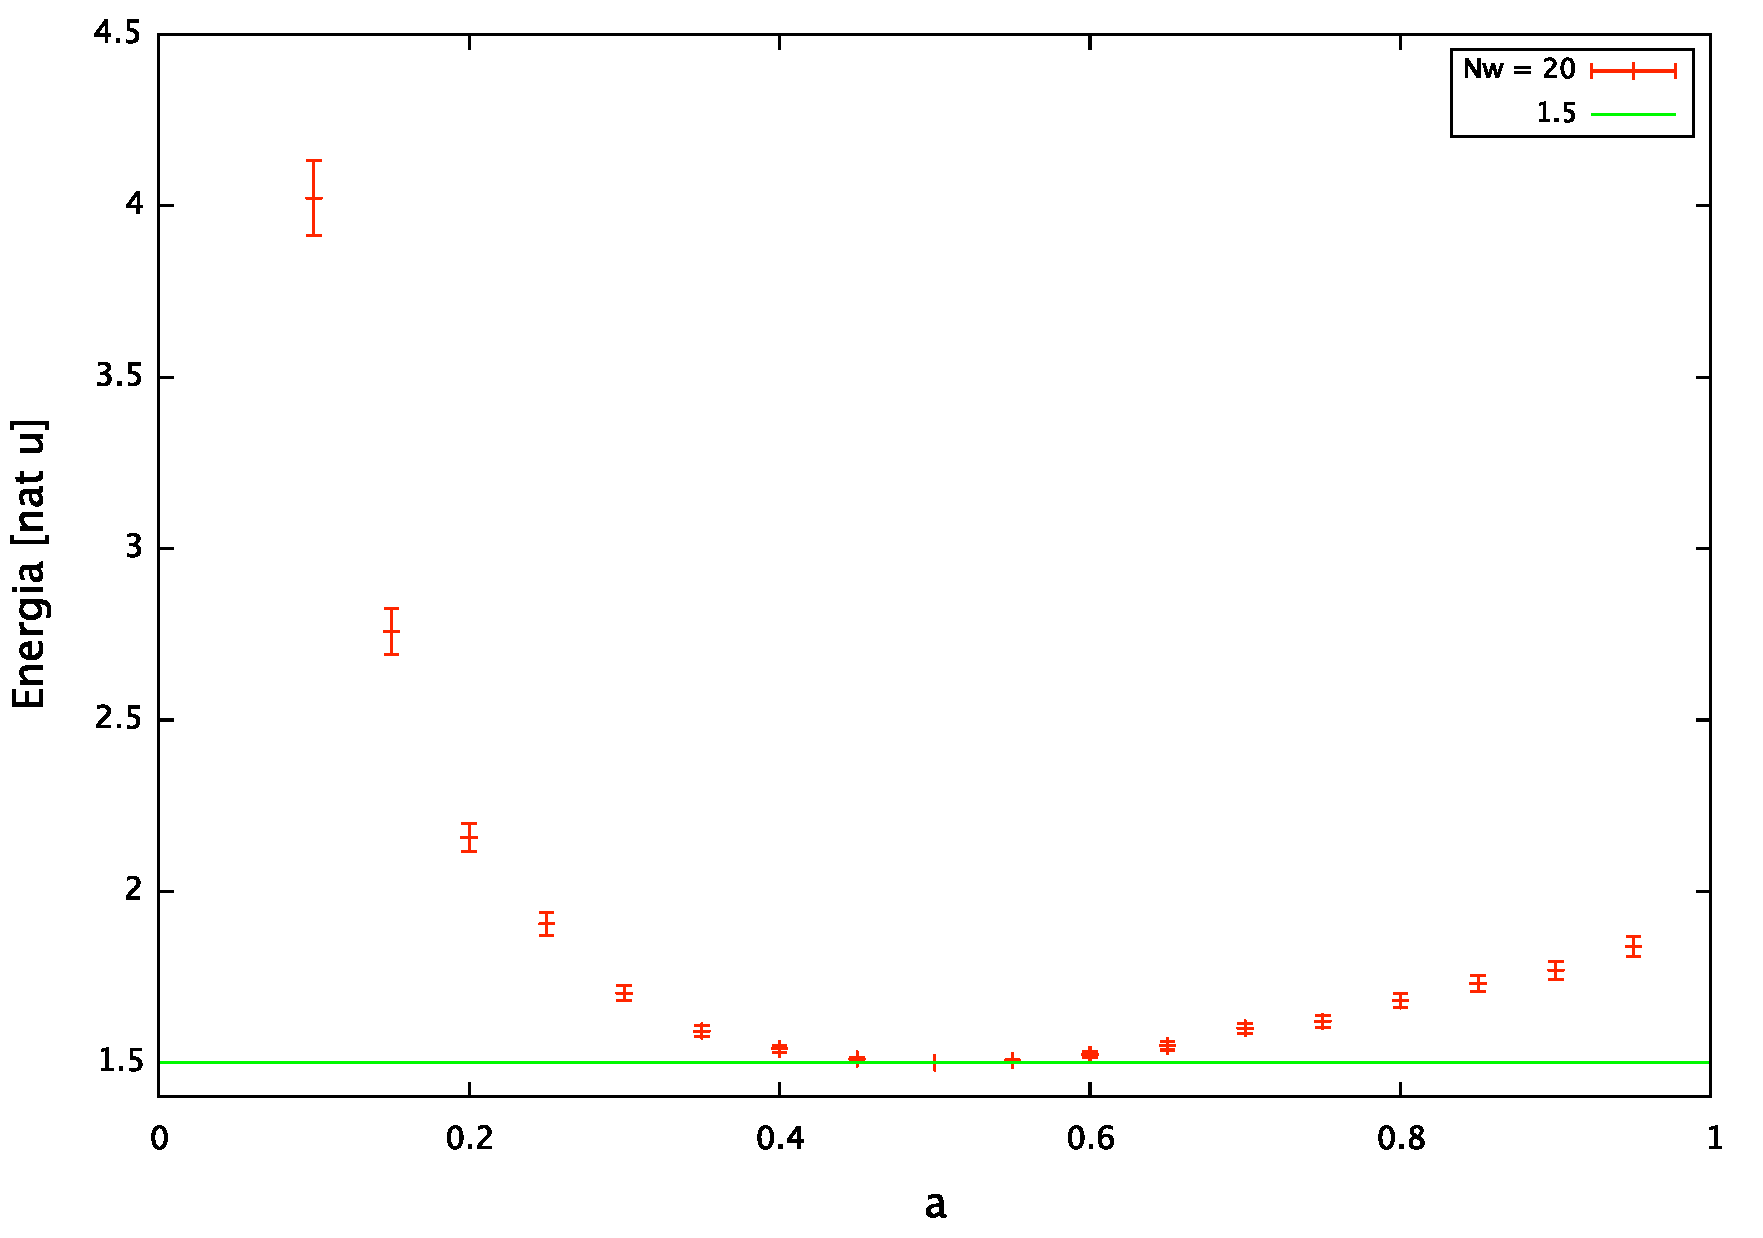
\includegraphics[scale=0.25]{Img/3dvar_1}}
\hspace{3mm}
\subfigure[$N=2$]
{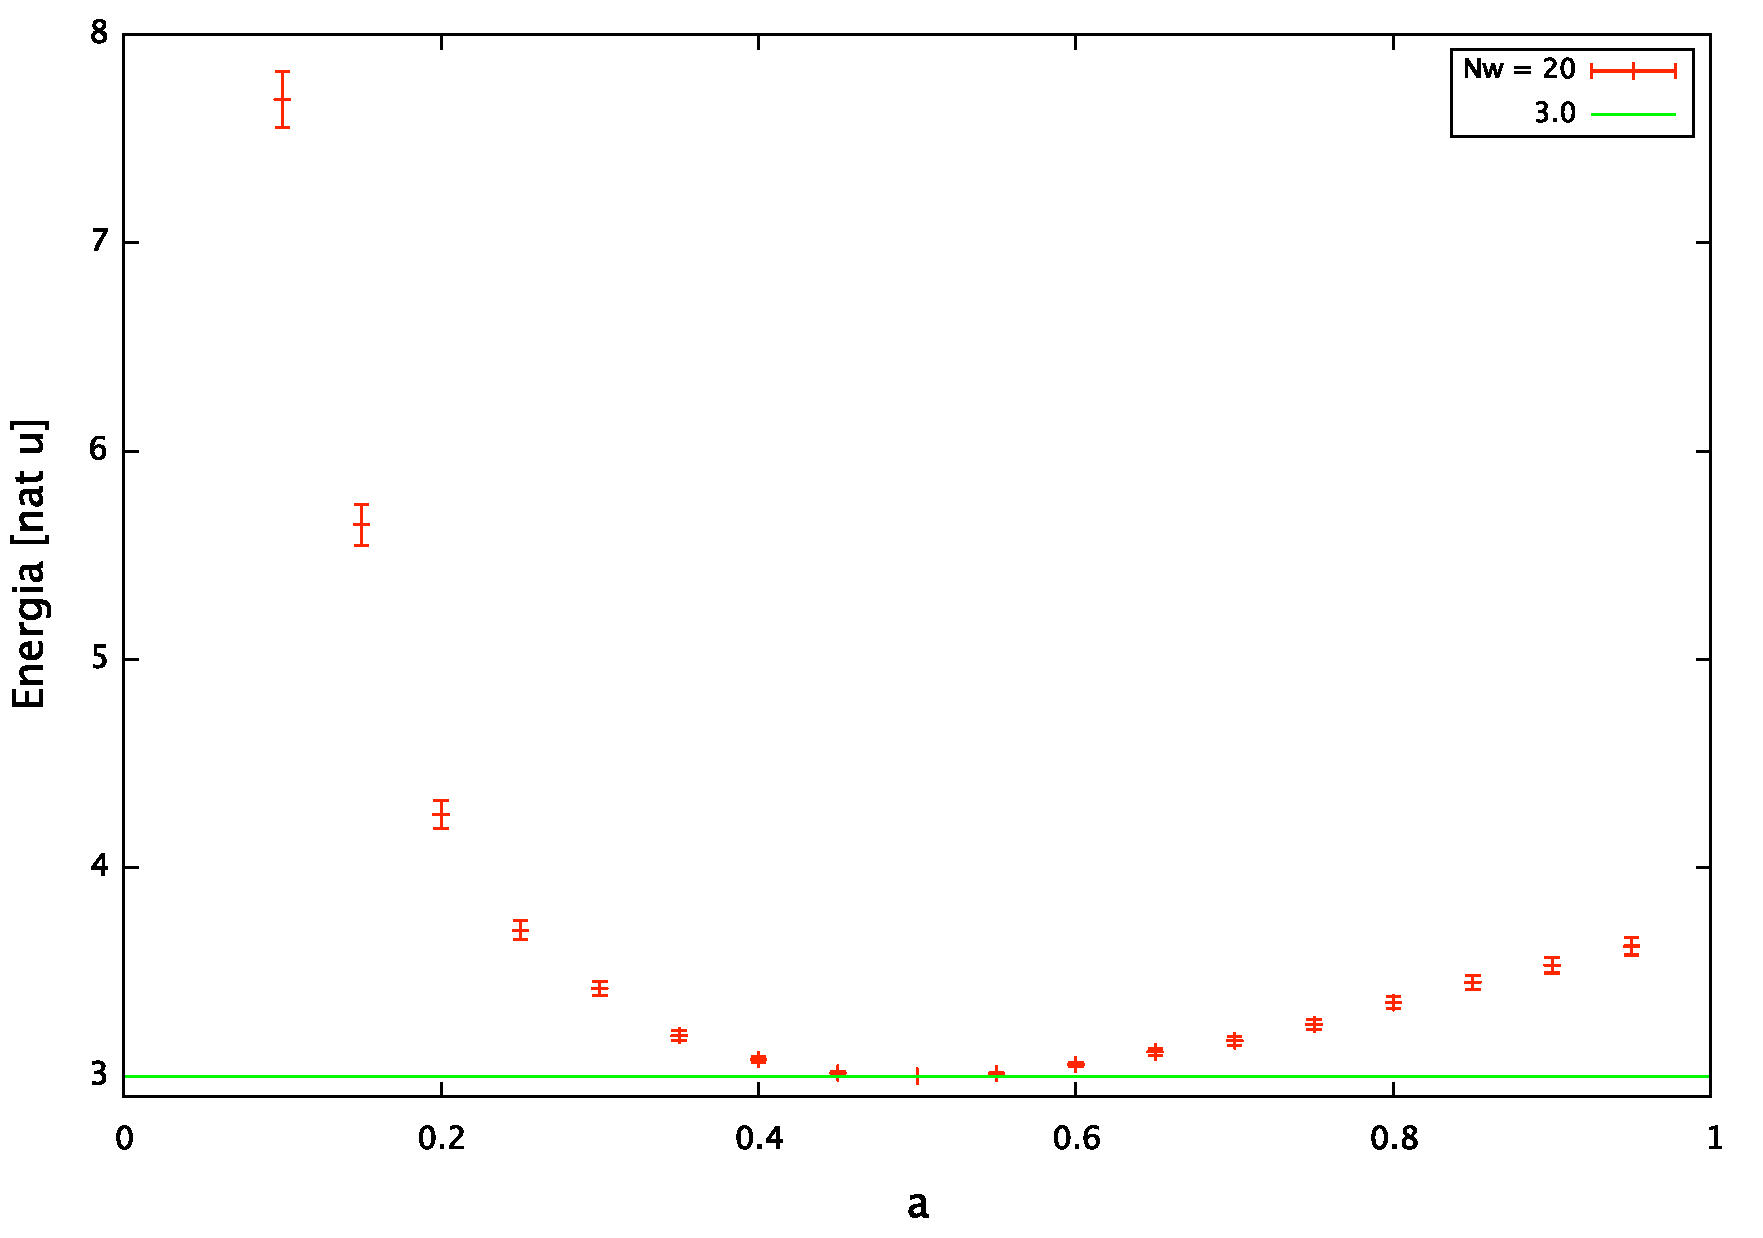
\includegraphics[scale=0.25]{Img/3dvar_2}}
\hspace{3mm}
\subfigure[$N=5$]
{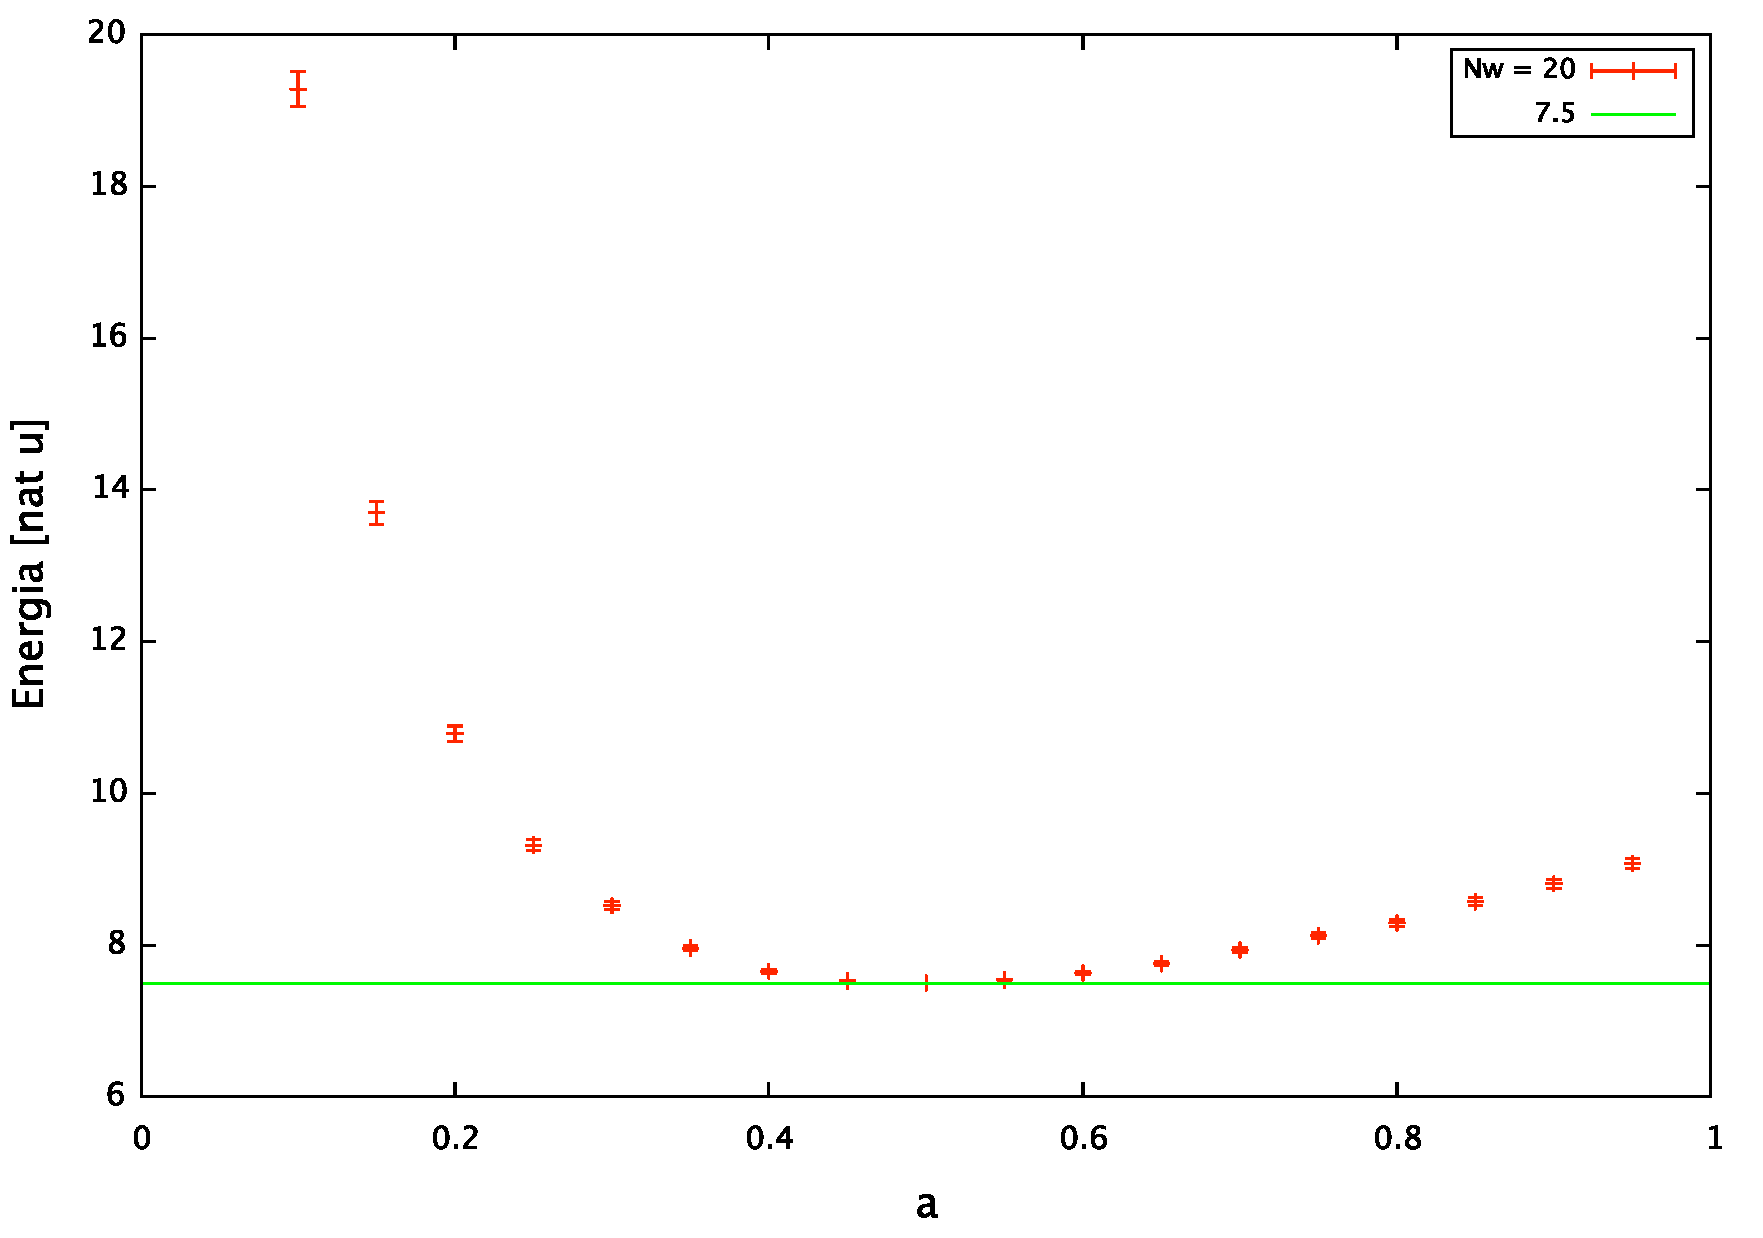
\includegraphics[scale=0.25]{Img/3dvar_5}}
\hspace{3mm}
\subfigure[$N=10$]
{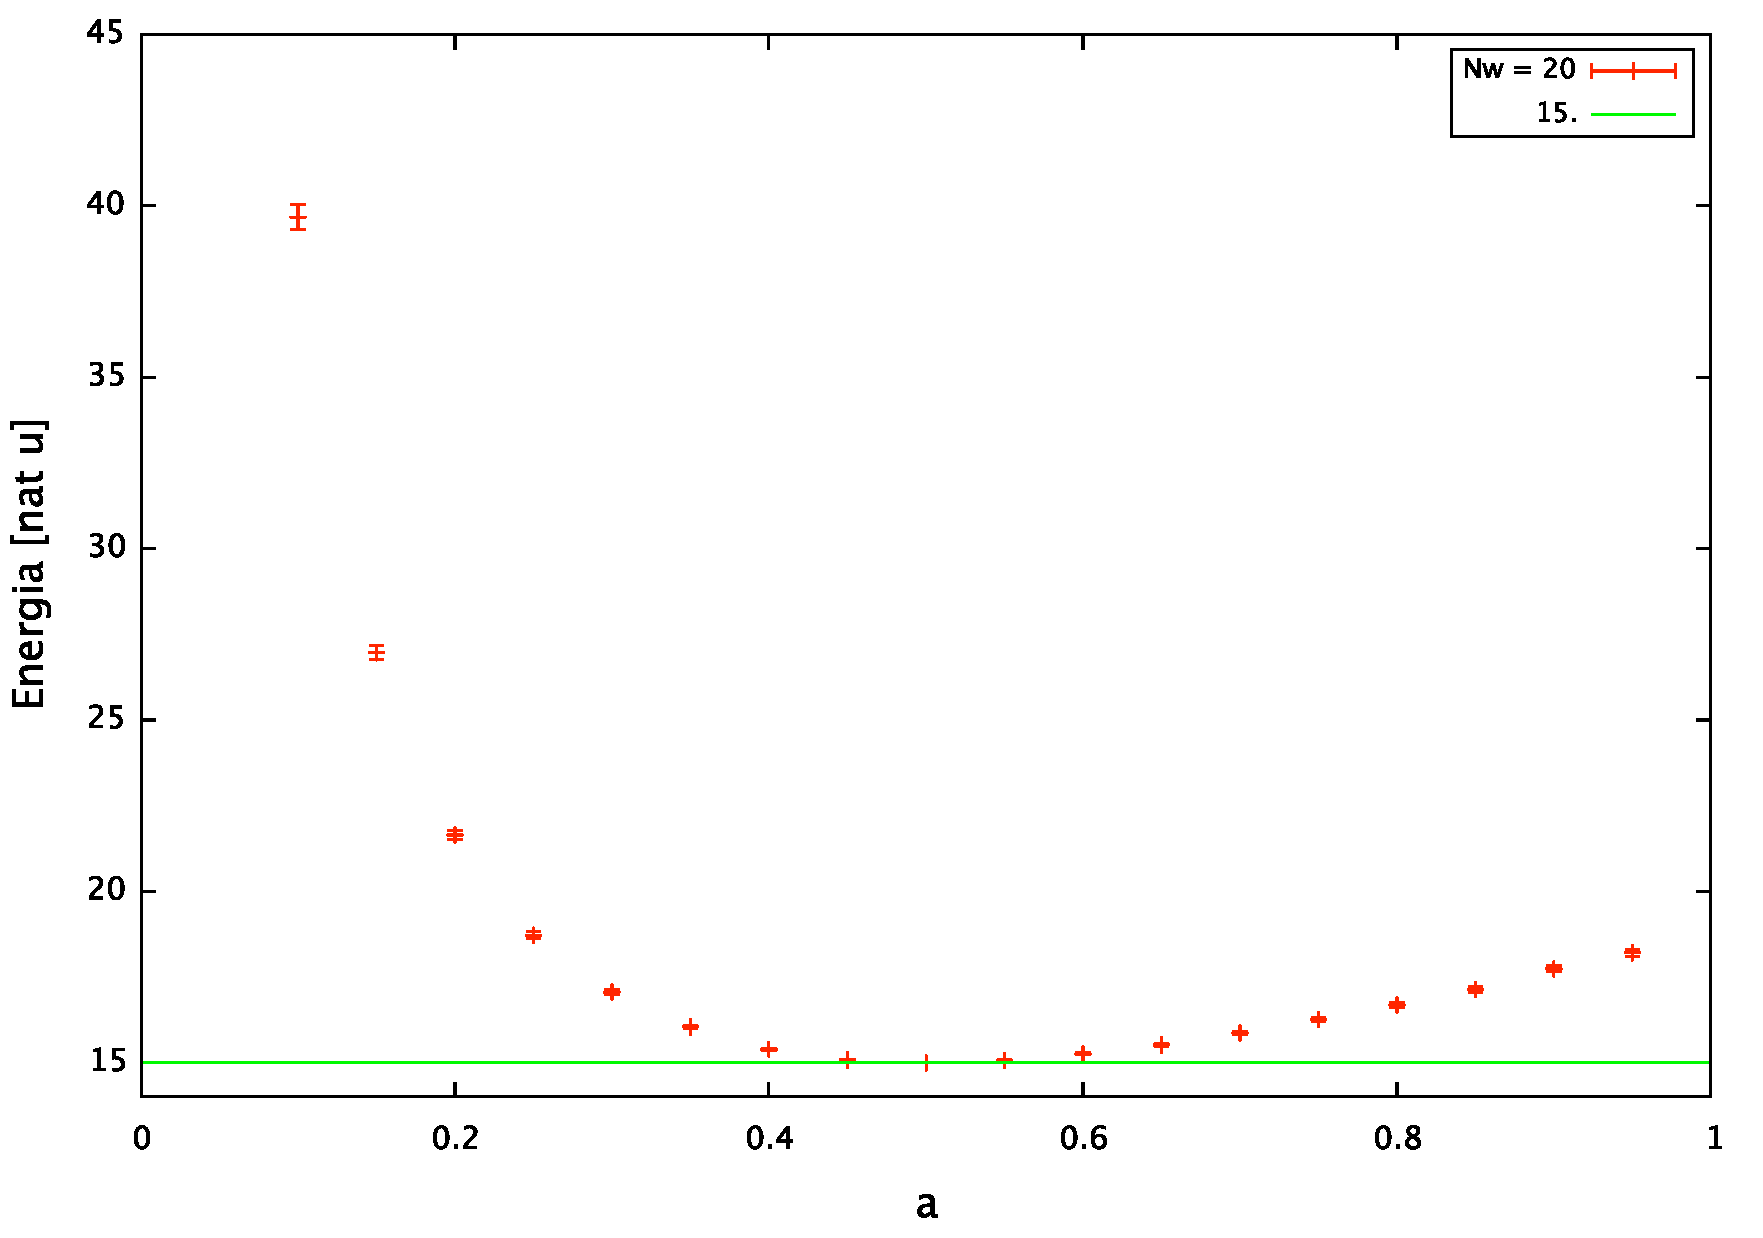
\includegraphics[scale=0.25]{Img/3dvar_10}}
\caption{Andamento $\langle E_{VMC}\rangle$ per diversi $a$ ed un diverso numero di particelle}
\end{figure}
Come atteso, utilizzando il criterio \eqref{20}, otteniamo che per $a=0.5$ le energie ottenute tramite VMC sono identiche alle previsioni teoriche, rispettivamente $E_0^{(1)}=1.5$, $E_0^{(2)}=3$, $E_0^{(5)}=7.5$ e $E_0^{(10)}=15$ e con varianza esattamente nulla. In Tab. (3) vengono mostrati alcuni valori rilevanti del calcolo VMC.
\begin{table}[!h]
\centering
\begin{tabular}{|c|c|c|c|c|c|c|}
\hline
$a$ & $E_0^{(2)}$ & $\sigma(E_0^{(2)})$ & $E_0^{(5)}$ & $\sigma(E_0^{(5)})$ & $E_0^{(10)}$ & $\sigma(E_0^{(10)})$ \\ \hline
0.1 &	7.7 & 0.1 & 19.3 & 0.2 & 39.7 & 0.4 \\ \hline
0.3  & 3.42 & 0.03 & 8.52 & 0.05 & 17.05 & 0.07 \\ \hline
0.5 	& 3.00 	 & 0.00 & 7.50 & 0.00 & 15.00 & 0.00 \\ \hline
0.7 	& 3.17 & 0.02 & 7.93 & 0.3 & 15.87 & 0.05 \\ \hline
\end{tabular}
\caption{Valori significativi dell'energia ottenuta tramite VMC per $E_T=3.$}
\end{table}
Concludiamo il test degli algoritmi VMC e DMC analizzando i risultati del DMC per 5 e 10 oscillatori armonici disaccoppiati in 3D. Fig. (9) mostra il confronto fra i risultati variazionali e quelli ottenuti dopo la diffusione con branching, mentre Fig. (10) mostra l'andamento dell'energia in funzione dei cicli di DMC per $a=0.3$. Come precedentemente osservato nel caso 1D con una particella, il meccanismo di proiezione in tempo immaginario del DMC permette di ottenere energie ragionevoli anche a partire da parametri variazionali molto lontani da quello corretto, e l'andamento convergente dell'energia è fortemente evidenziato dal comportamento in Fig. (10). Possiamo considerare dunque che il test preliminare dell'algoritmo sia andato a buon fine ed applicare il meccanismo al problema più complicato dell'elio liquido. 
 \begin{figure}[!h]
\centering
\subfigure[$N=5$]
{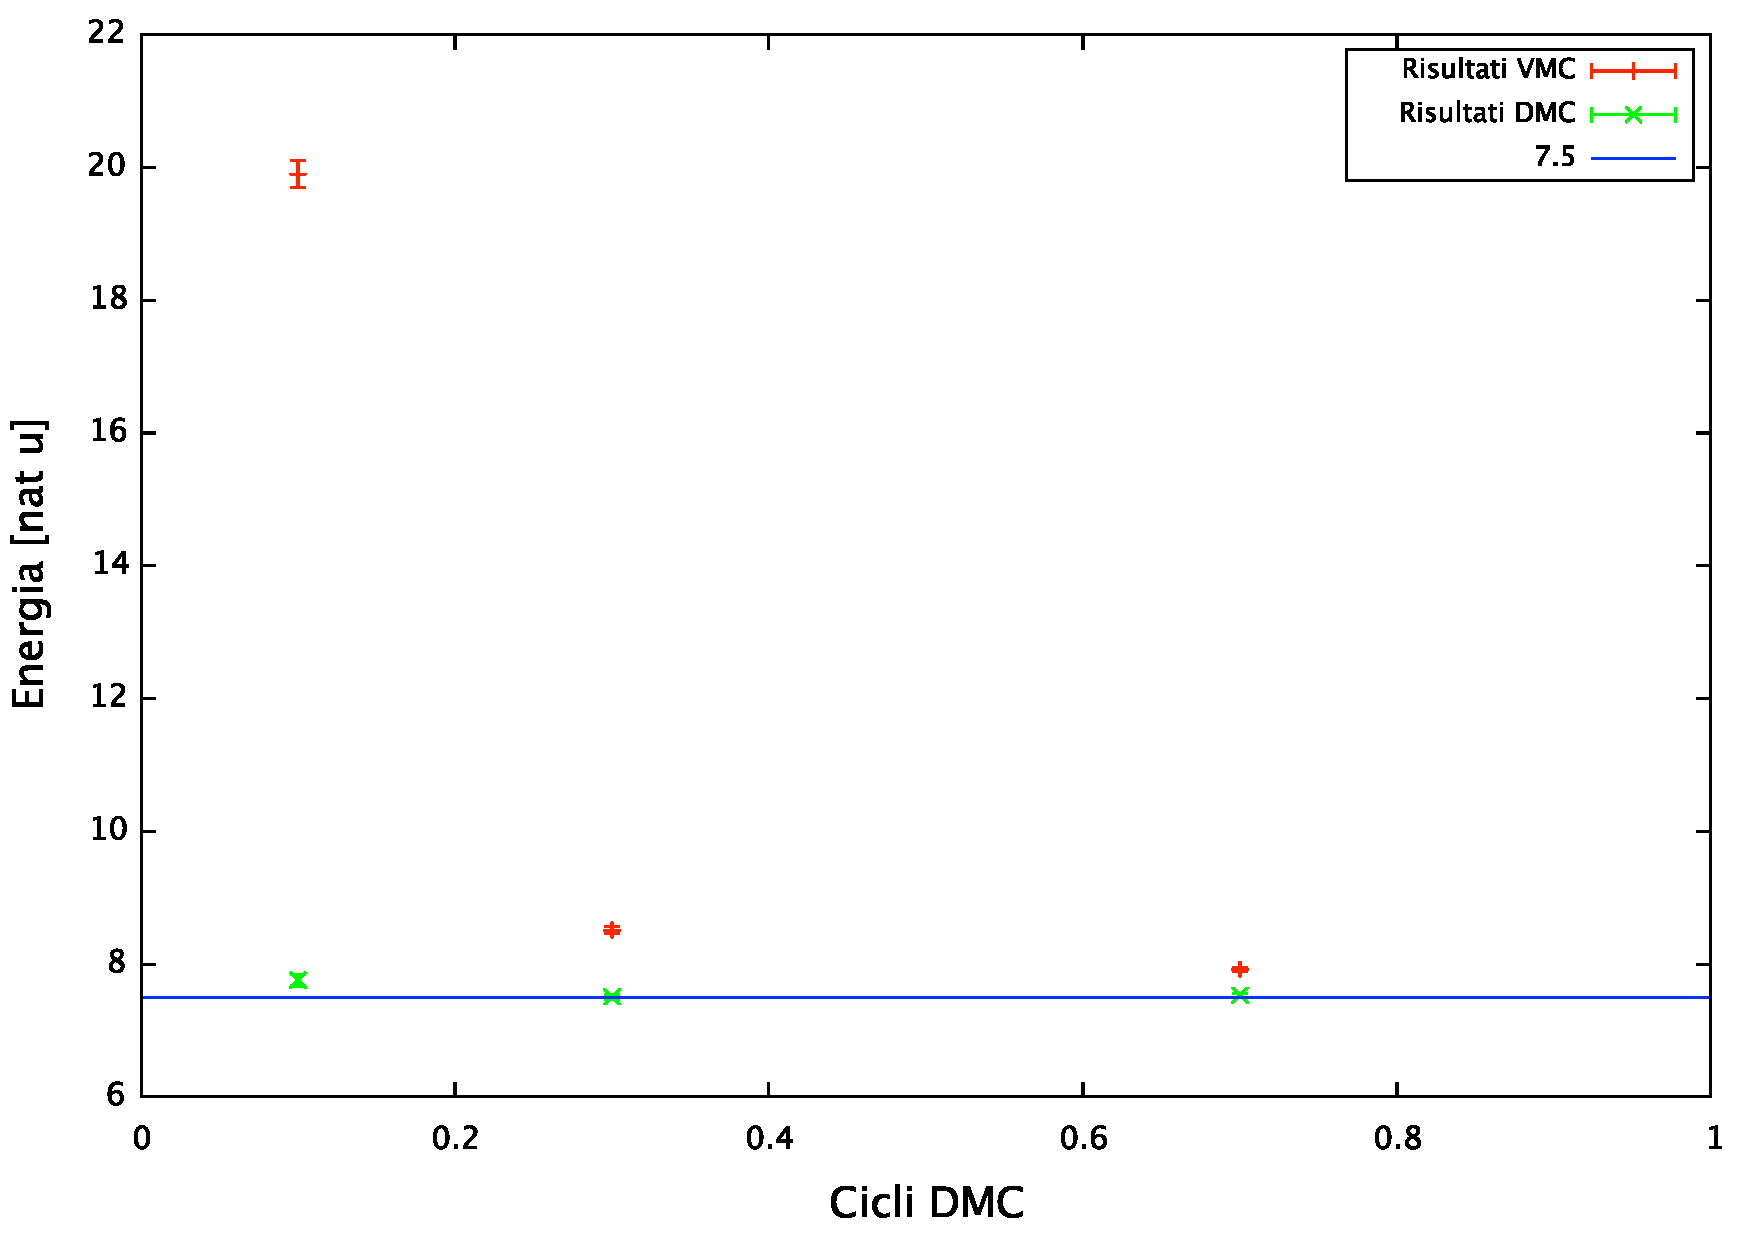
\includegraphics[scale=0.25]{Img/dmc_var_5}}
\hspace{3mm}
\subfigure[$N=10$]
{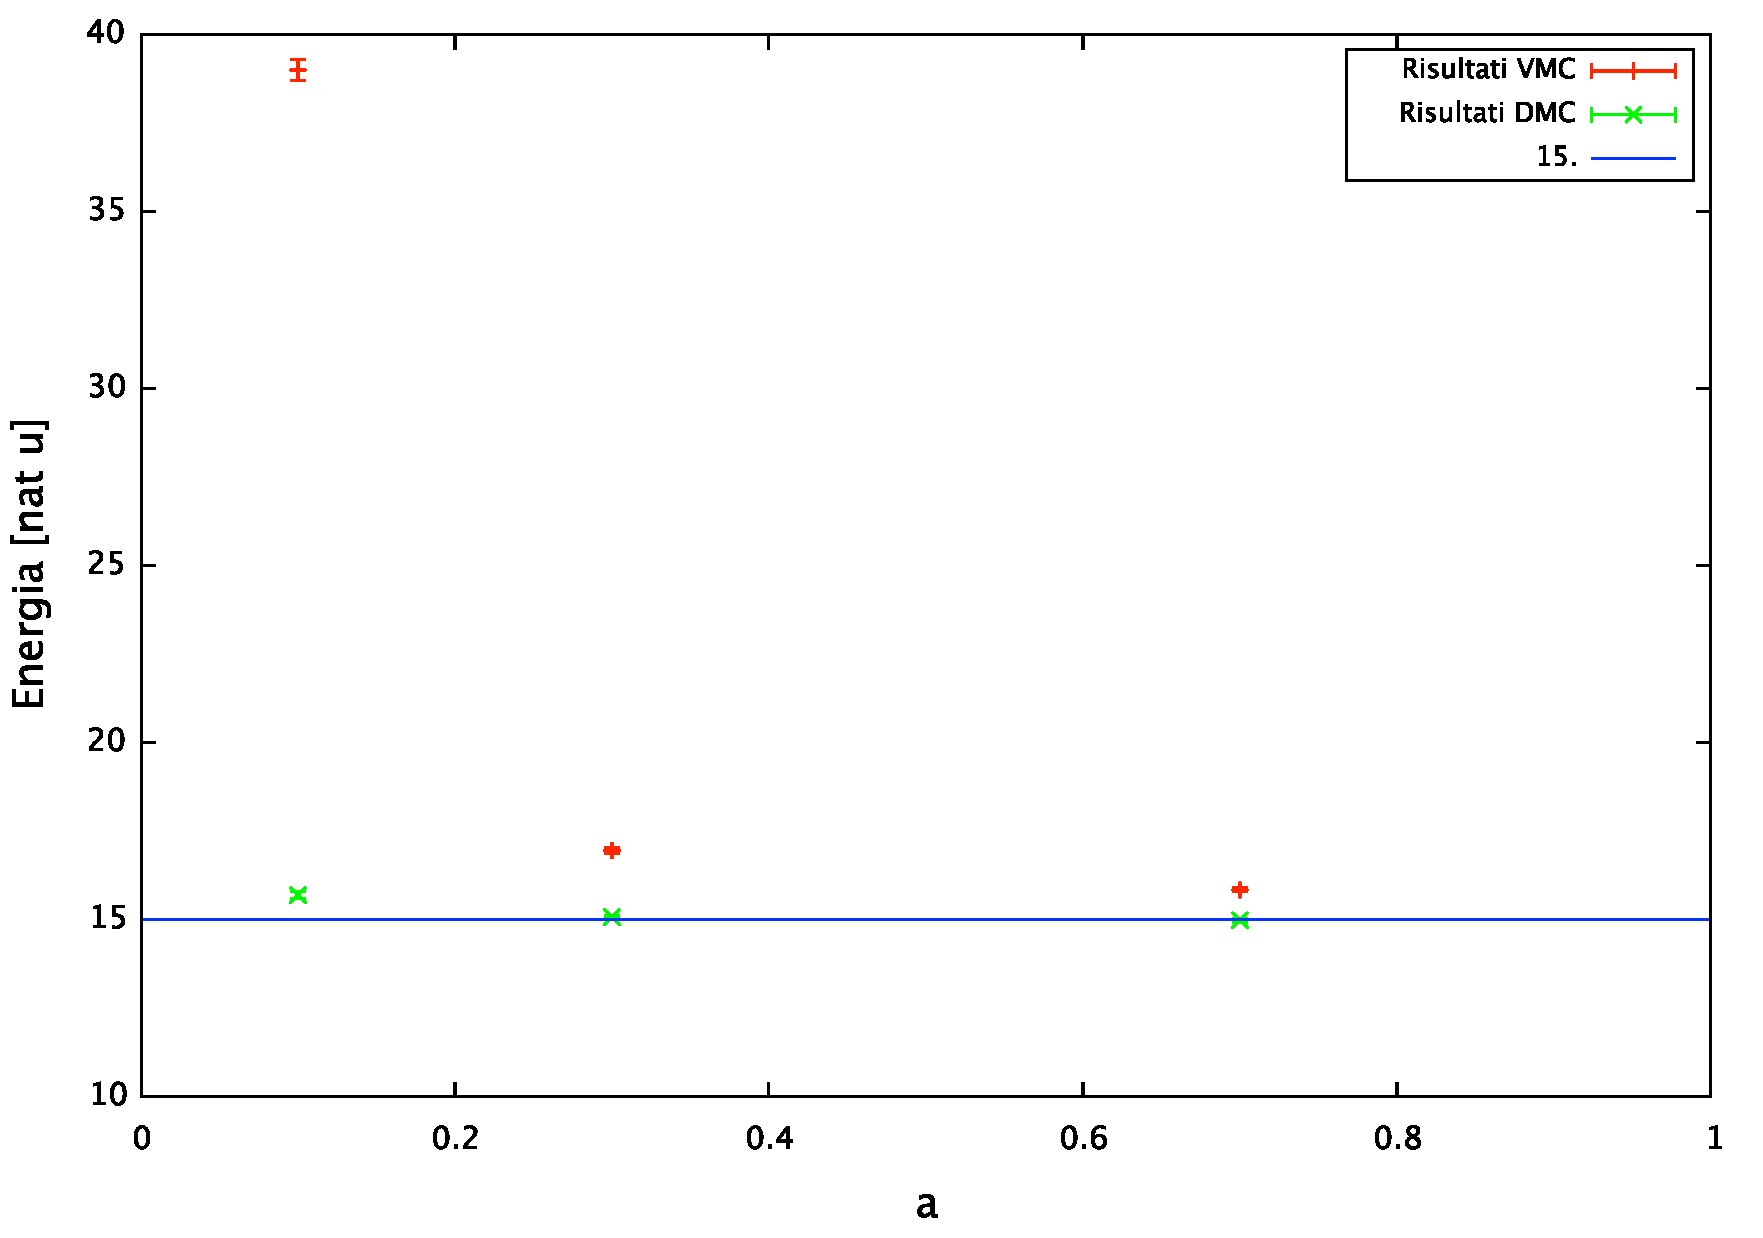
\includegraphics[scale=0.25]{Img/dmc_var_10}}
\caption{Confronto fra risultato VMC e risultato DMC per gli stessi $a$}
\end{figure}
 \begin{figure}[!h]
\centering
\subfigure[$N=5$]
{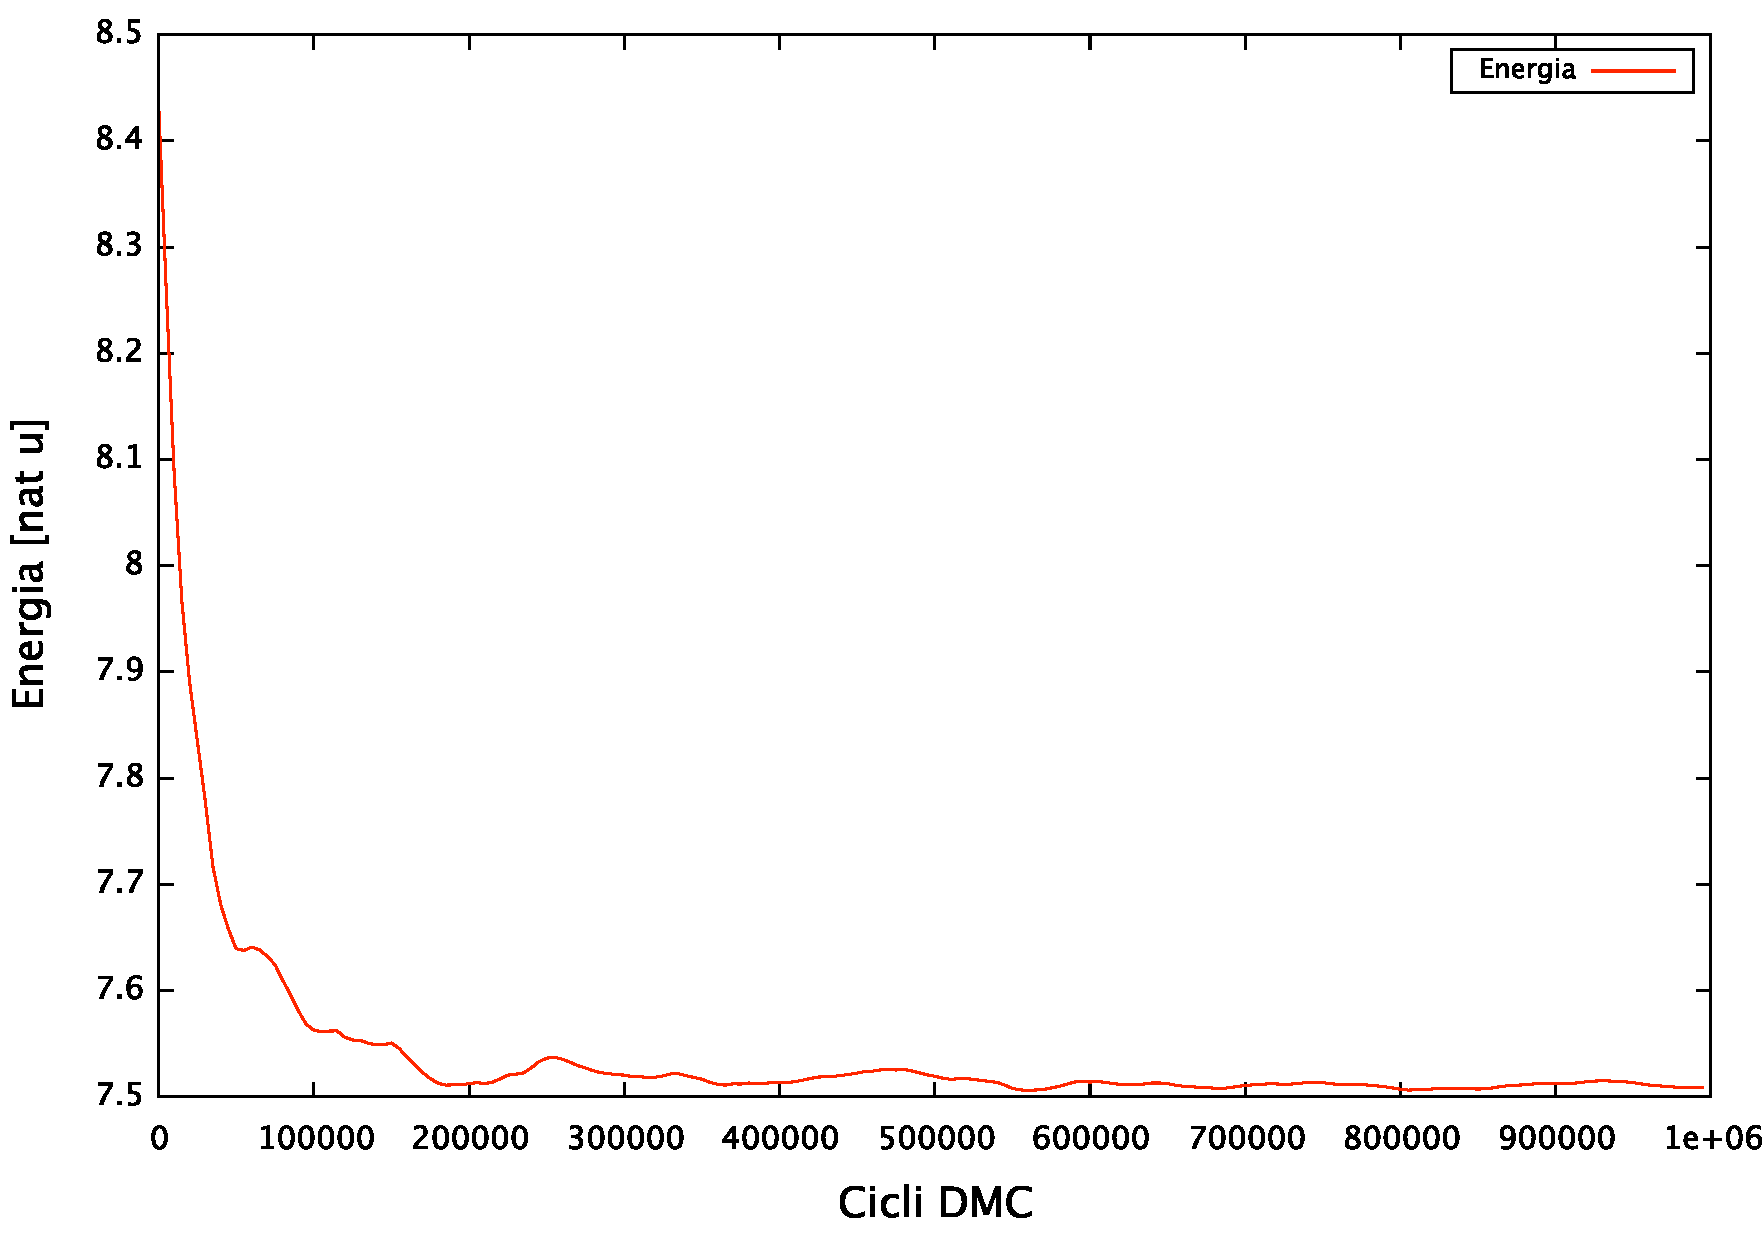
\includegraphics[scale=0.25]{Img/e_5}}
\hspace{3mm}
\subfigure[$N=10$]
{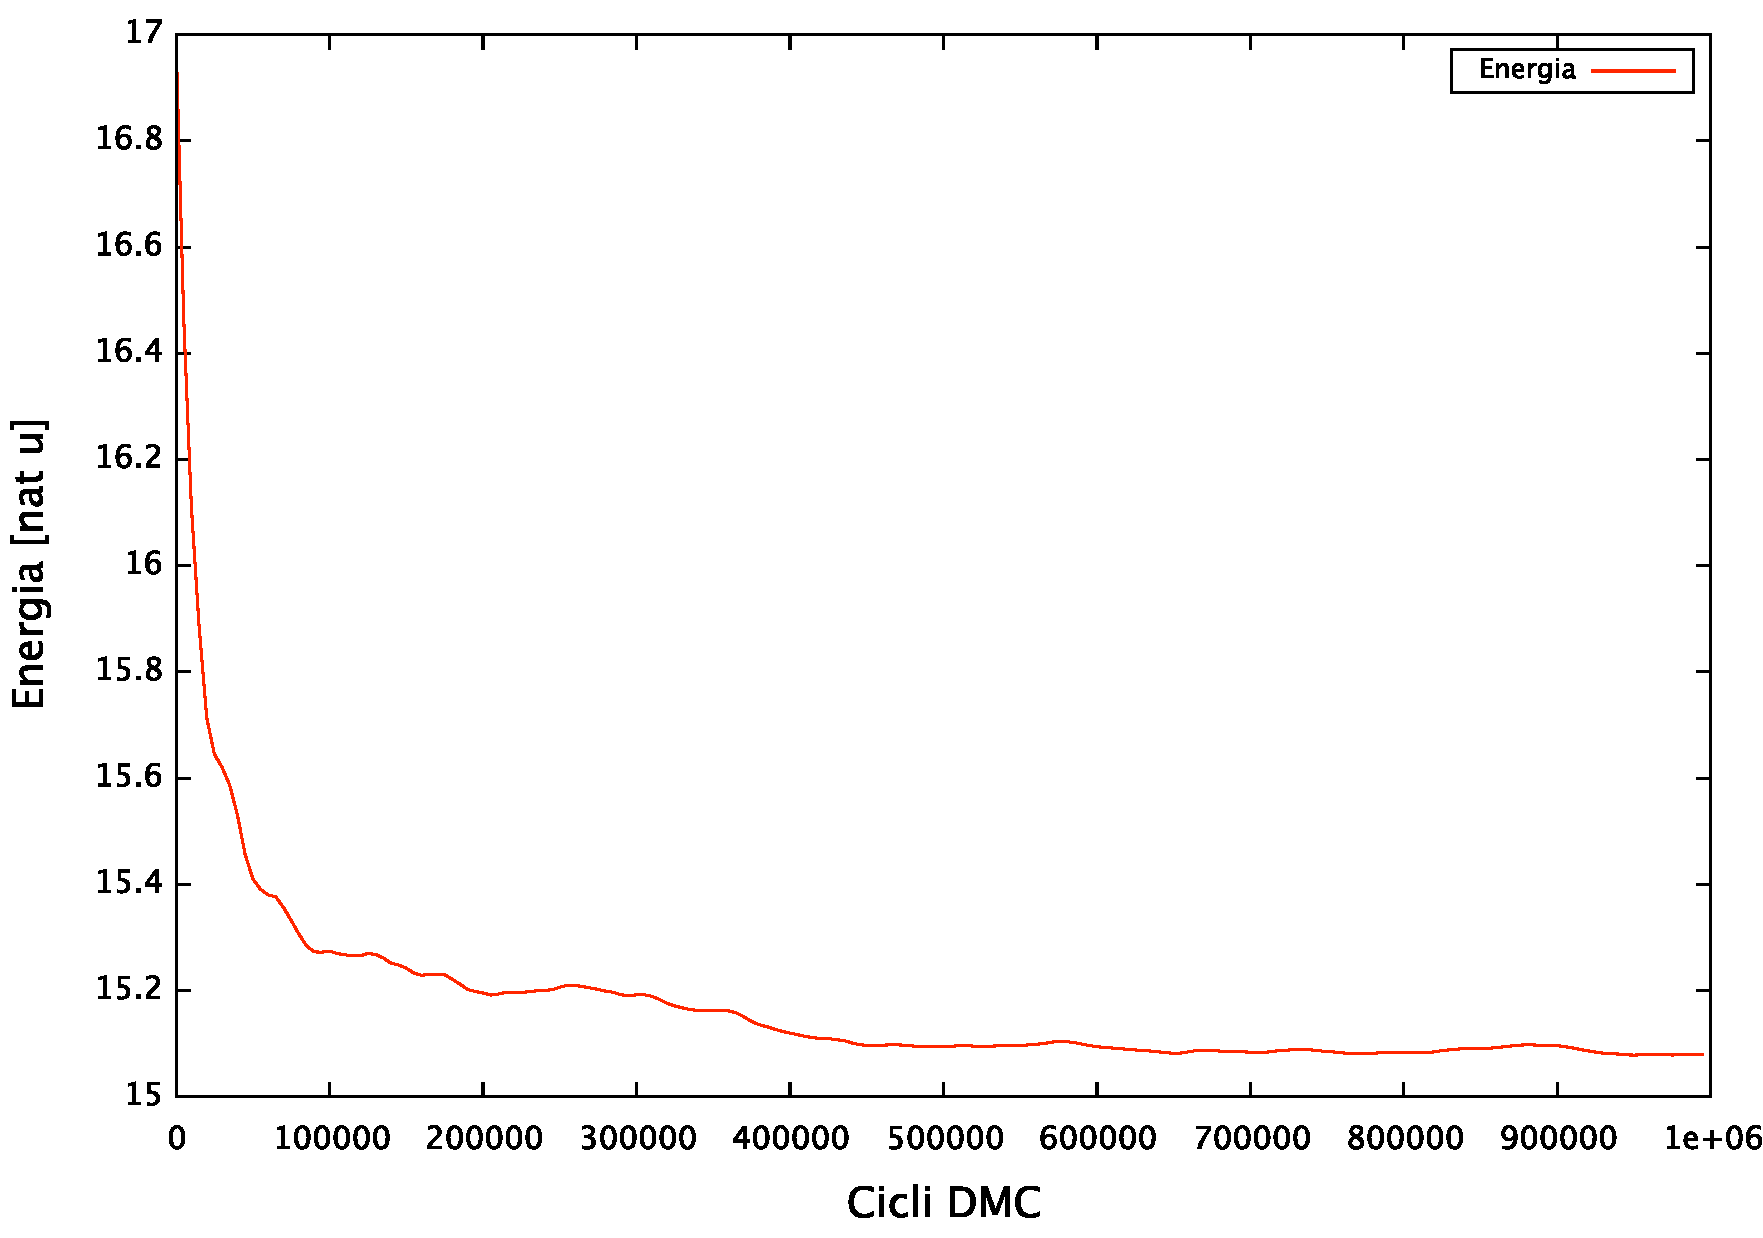
\includegraphics[scale=0.25]{Img/e_10}}
\caption{Andamento dell'energia in funzione del numero di cicli DMC, per $a=0.3$}
\end{figure}

\section{Elio liquido}
\subsection{Preparazione: energia locale, pseudoforza e unità ridotte}
Il problema dell'elio liquido è (come da titolo) descritto dalla seguente Hamiltoniana:
\begin{equation}
\mathcal{H} = -\frac{\hbar^2}{2m}\sum_{i=1}^N \nabla_i^2 + \sum_{i=1}^N\frac{1}{2}m\omega^2\textbf{r}_i^2 + \sum_{i<j}4\varepsilon \left[ \left(\frac{\sigma}{r_{ij}}\right)^{12}- \left(\frac{\sigma}{r_{ij}}\right)^6 \right]
\end{equation}
La natura a due corpi dell'Hamiltoniana suggerisce la necessità di utilizzare una funzione d'onda trial non banale. Una possibilità è quella fornita dall'\emph{espansione di Wu-Feenberg}, che propone di fattorizzare la funzione d'onda come il prodotto di due contributi, uno a un corpo ed uno a due corpi:
\begin{equation}
\psi_T(\textbf{r}_1,\ldots,\textbf{r}_N) = \prod_{i=1}^N \phi(\textbf{r}_i)\prod_{i<j}f^{(2)}(r_{ij})
\end{equation}
Senza perdita di generalità, possiamo riscrivere
\[
\prod_{i<j}f^{(2)}(r_{ij}) = \exp\left[ -\frac{1}{2}\sum_{i<j}u^{(2)}(r_{ij})\right]
\]
e ci chiediamo: come deve essere fatta $u^{(2)}(r_{ij})$ perchè la condizione di cuspide sia soddisfatta? Più precisamente, dobbiamo far sì che sia soddisfatta
\begin{equation}
\lim_{R\to R_0}\frac{\mathcal{H}\psi_T(R)}{\psi_T(R)}< +\infty
\end{equation}
Osserviamo che
\[
V(R) = 4\varepsilon \sum_{i<j}\left[ \left(\frac{\sigma}{r_{ij}}\right)^{12}- \left(\frac{\sigma}{r_{ij}}\right)^6 \right] \xrightarrow[R \to R_0]{} 4\varepsilon \sum_{i<j}\left(\frac{\sigma}{r_{ij}}\right)^{12}
\]
Focalizziamo la nostra attenzione sulla componente a due corpi della funzione d'onda e mettiamo in un sistema di coordinate relative: dobbiamo verificare che per per ciascuna coppia valga
\[
\lim_{r \to 0} \left[ -\frac{\hbar^2}{2\mu}\frac{\nabla^2 e^{-\frac{1}{2}u^{(2)}(r)}}{e^{-\frac{1}{2}u^{(2)}(r)}} +  4\varepsilon\left(\frac{\sigma}{r_{ij}}\right)^{12}\right] < +\infty
\]
Si ottiene
\[
\begin{split}
\frac{\nabla^2 e^{-\frac{1}{2}u^{(2)}(r)}}{e^{-\frac{1}{2}u^{(2)}(r)}} &= \frac{1}{e^{-\frac{1}{2}u^{(2)}(r)}}\frac{d^2}{dr^2}e^{-\frac{1}{2}u^{(2)}(r)} + \frac{2}{re^{-\frac{1}{2}u^{(2)}(r)}}\frac{d}{dr}e^{-\frac{1}{2}u^{(2)}(r)} \\
&= -\frac{1}{2}\frac{d^2u^{(2)}(r)}{dr^2}+\frac{1}{4}\left( \frac{du^{(2)}(r)}{dr}\right)^2 - \frac{1}{r}\frac{du^{(2)}(r)}{dr}
\end{split}
\]
da cui
\[
\lim_{r \to 0} \left[ -\frac{\hbar^2}{2\mu}\left( -\frac{1}{2}\frac{d^2u^{(2)}(r)}{dr^2}+\frac{1}{4}\left( \frac{du^{(2)}(r)}{dr}\right)^2 - \frac{1}{r}\frac{du^{(2)}(r)}{dr} \right) +  4\varepsilon\left(\frac{\sigma}{r_{ij}}\right)^{12}\right] < +\infty
\]
Come possibile espressione analitica di $u^{(2)}(r)$ si può proporre
\begin{equation}
u^{(2)}(r) = \left( \frac{b}{r} \right)^m
\end{equation}
con $b$ parametro variazionale che determineremo tramite VMC ed $m$ esponente da determinare per soddisfare la condizione di cuspide. Si ottiene
\[
\frac{du^{(2)}(r)}{dr} = -m\frac{b^m}{r^{m+1}} \qquad \frac{d^2u^{(2)}(r)}{dr^2} = m(m+1)\frac{b^m}{r^{m+2}}
\]
da cui, raccogliendo e rimaneggiando i termini
\begin{equation}
\lim_{r \to 0} \left[ -\frac{\hbar^2}{2\mu}\frac{m^2b^{2m}}{4r^{2m+2}}+4\varepsilon\left(\frac{\sigma}{r_{ij}}\right)^{12} \right] < +\infty
\end{equation}
L'unica potenza che permette di soddisfare la condizione di cuspide è $m=5$. Ne deduciamo allora che una buona funzione d'onda trial per il calcolo Monte Carlo è data da
\begin{equation}
\psi_T(\textbf{r}_1,\ldots,\textbf{r}_N) = \prod_{i=1}^Ne^{ -a\textbf{r}_i^2} \prod_{i<j=1}^N e^{-\frac{1}{2}\left( \frac{b}{r_{ij}} \right)^5}
\end{equation}
Una volta definita la funzione d'onda trial che vogliamo utilizzare, definiamo delle unità ridotte con cui riscrivere l'Hamiltoniana di partenza. Cominciamo fissando un'unità di energia ed una di lunghezza. Possiamo definire l'unità di energia $\varepsilon_0$ come $k_B \varepsilon_0 = \hbar \omega$, mentre come lunghezza tipica del sistema possiamo utilizzare la lunghezza di oscillatore armonico (in letteratura di materia condensata è nota come $a_{ho}^2$) 
\[
\sigma_0^2 = \frac{\hbar}{m\omega} = \frac{\hbar\omega}{m\omega^2} = \frac{k_B\varepsilon_0}{m\omega^2}
\]
Fissiamo $\sigma_0$ come una frazione di $\sigma$:
\begin{equation}
\sigma = \Lambda \sigma_0
\end{equation}
con $\Lambda$ parametro da fissare, ed $\varepsilon_0$ come frazione di $\varepsilon$:
\begin{equation}
\varepsilon = \alpha \varepsilon_0
\end{equation}
In queste unità l'Hamiltoniana diventa
\begin{equation}
\mathcal{\tilde{H}} = -\frac{1}{2}\sum_{i=1}^N \tilde{\nabla}_i^2 + \sum_{i=1}^N\frac{1}{2}\tilde{\textbf{r}}_i^2 + \sum_{i<j}4\alpha \left[ \left(\frac{\Lambda}{\tilde{r}_{ij}}\right)^{12}- \left(\frac{\Lambda}{\tilde{r}_{ij}}\right)^6 \right]
\end{equation}
dove abbiamo indicato con la tilde le quantità riscalate. Fissato, ad esempio, $\Lambda = 0.25$, possiamo calcolare $\alpha$ di conseguenza, noto il fatto che, per $^{4}$He $\varepsilon =$10.4K e $\sigma=$2.556\angstrom: 
\[
\varepsilon_0 = \frac{\hbar^2}{m\sigma_0^2k_B} = 0.1159\text{K} \Rightarrow \alpha = \frac{\varepsilon}{\varepsilon_0} = 89.7325
\]
La scelta di $\Lambda$ è compatibile con il richiedere che il fondo della buca armonica possa contenere più di una particella. 
\end{document}